\documentclass[11pt]{article}

% === Packages ===
\usepackage[utf8]{inputenc}
\usepackage[T1]{fontenc}
\usepackage{amsmath,amssymb,amsthm}
\usepackage{booktabs}
\usepackage{graphicx}
\usepackage{hyperref}
\usepackage[a4paper,margin=1in]{geometry}
\usepackage[numbers,sort&compress]{natbib}
\setcitestyle{numbers}
\usepackage{xcolor}
\usepackage{enumitem}
\usepackage{tabularx}

% === Theorem environments ===
\newtheorem{theorem}{Theorem}[section]
\newtheorem{lemma}[theorem]{Lemma}
\newtheorem{proposition}[theorem]{Proposition}
\theoremstyle{definition}
\newtheorem{definition}[theorem]{Definition}
\theoremstyle{remark}
\newtheorem{remark}[theorem]{Remark}

% === Metadata ===
\title{Context Is Inventory:\\ A Rent-or-Buy Model for Prompt-Cached LLM Sessions}
\author{Longju Cheng}
\date{July 2026}

\begin{document}
\maketitle

\begin{abstract}
Prompt caching in large language model (LLM) APIs introduces a structural asymmetry: cached reads are an order of magnitude cheaper than uncached writes, creating a ``rent-or-buy'' trade-off for every token of accumulated session context. We show that this trade-off maps exactly onto two classic models from inventory theory---the Economic Order Quantity (EOQ) and the ski-rental problem---yielding a unified cost framework for LLM session economics. The mapping produces three results. First, it proves that under any prompt-caching pricing scheme, the share of per-turn cost addressable by restart timing has a mathematical supremum of $\sqrt{2}-1\approx 41.4\%$; realized values range from $\sim$32\% to $\sim$41\% depending on the provider's cost ratio $R$, with high-$R$ providers (DeepSeek V4 Pro, $R{\approx}120$) operating near the bound. Second, it derives a closed-form regret function $(k + 1/k - 2)/2 \cdot A(n^*)$ that gives the exact cost of any deviation from the optimal restart interval, and identifies the structural interface through which the learning-augmented ski-rental framework could incorporate operator-supplied foresight ($\alpha$, $H$) when a concrete instantiation is developed. Third, we present preliminary empirical measurements ($n=1$, author-as-subject) from real session transcripts: per-turn growth $g(t)$ is stationary (100\% of segments reject the unit-root null) with cross-plateau-stable rates (median 644 tok/turn); cumulative context $L(t)$, while integrated ($I(1)$, mechanically inflating $R^2 \ge 0.957$), exhibits consistent linear plateaus after fold-jump removal (plateau $R^2 \ge 0.975$); a per-turn forward reconstruction recovers $91\%$ of billed costs across 20~days; and provider TTL expiration collapses the effective read/write cost ratio in orchestrator workflows. The reconstruction rules were calibrated on the same billing month, so the 91\% recovery is in-sample; cross-operator generalization remains untested. The framework treats restart timing as a \emph{guardrail}---preventing unbounded tail-regret---rather than an \emph{optimizer} chasing a fundamentally shallow optimum. We release an open-source tool that implements the model as live cost instrumentation for LLM sessions.
\end{abstract}

% ======================================================================
\section{Introduction}
% ======================================================================

Prompt caching has become a standard feature of production LLM APIs. Anthropic, OpenAI, DeepSeek, and Google all offer mechanisms by which repeated token prefixes incur only a fraction of the base input price---typically $10\%$ for a cache hit, versus $100\%$ or $125\%$ for a cache miss \citep{anthropic2025caching, deepseek2025caching, openai2025caching}. The economic intuition is straightforward: cache what repeats, pay full price for what does not.

But this intuition masks a subtler dynamic. Every turn of an LLM session \emph{grows} the context. Tool outputs, conversation history, code snippets, test results---all accumulate. And because each subsequent turn must re-process the accumulated prefix, the rent on every byte of history compounds turn after turn. A session that runs $n$ turns pays rent on its first turn's output $n$ times. The cost of \emph{not} restarting is an invisible slope.

Meanwhile, restarting is not free. A fresh session must rebuild its working context---system prompt, tool definitions, domain vocabulary---incurring cache-miss costs on what was previously a warm prefix. The restart decision is precisely a rent-or-buy trade-off: keep running and pay incremental holding costs on accumulated context, or restart and pay a one-time rebuild cost.

This paper shows that this trade-off is not merely analogous to classical inventory problems---it is \emph{structurally identical}. Under stateless, flow-billed (cost is per-token per-request, not per unit time) prompt-caching APIs, the per-turn cost function of an LLM session is isomorphic to the Economic Order Quantity (EOQ) cost function \citep{harris1913}, and the restart decision is isomorphic to the ski-rental (rent-or-buy) online decision problem \citep{karlin1994}. The mapping yields a unified cost model with three contributions:

\begin{enumerate}[leftmargin=*,itemsep=0pt,topsep=0pt]
\item \textbf{A structural upper bound.} At the optimal restart interval, the share of per-turn cost that restart timing can influence never exceeds $\sqrt{2}-1 \approx 41.4\%$. The floor is mathematical, not empirical---a direct consequence of the AM-GM inequality applied to the two-term cost decomposition developed in Section~3.
\item \textbf{A bounded-regret guarantee with a human-in-the-loop mapping.} Deviation from the optimal restart interval $n^*$ by a factor $k = n/n^*$ incurs exact regret $(k + 1/k - 2)/2 \cdot A(n^*)$, where $A(n^*)$ is the movable cost at the optimum. The regret function is convex and unbounded as $k \to \infty$, making the cost of neglect arbitrarily large while the cost of moderate timing error ($k \in [0.5, 2]$) is at most 5--10\% of per-turn cost---a structural consequence of the EOQ flat-valley property. When the human operator supplies a prediction of remaining task horizon $H$ and task-carry relevance $\alpha$, the policy would upgrade to the learning-augmented ski-rental framework of \citet{purohit2018}, trading consistency for robustness via a single parameter $\lambda$.
\item \textbf{Preliminary data collection.} We instrument real LLM session transcripts from a single operator (the author, $n=1$) and report: (a) per-turn growth $g(t)$ is stationary (100\% unit-root rejection) and cross-plateau stable (median $k_{\text{stable}} \approx 644$ tok/turn, p25--p75: 532--871); cumulative $L(t)$ is $I(1)$ (mechanically high $R^2 \ge 0.957$), but after fold-jump removal exhibits linear plateaus with $R^2 \ge 0.975$; (b) a per-turn forward reconstruction recovers $91\%$ of billed DeepSeek costs (median across 20~days, all three cost components aligned; in-sample, rules fit on the same billing month); and (c) provider TTL expiration collapses the effective read/write cost ratio by up to $3.7\times$ in orchestrator workflows (measured; see Table~\ref{tab:ttl}). These measurements are preliminary---cross-operator and out-of-sample data are not yet available---but they demonstrate that the model's structural quantities are observable in real billing telemetry.
\end{enumerate}

The overarching thesis is that the model is a \emph{guardrail}, not an \emph{optimizer}: the optimum is shallow, but the tail is infinite. The $41.4\%$ bound limits what precise timing can achieve; the regret function $(k+1/k-2)/2\cdot A(n^*)$ quantifies the exact cost of structural under-reaction, growing unboundedly as $k\to\infty$. Between these two boundaries lies a remarkably flat cost curve---the ``flat valley'' of EOQ sensitivity analysis---in which timing precision contributes less than intuition expects, while catastrophic neglect costs unboundedly more. Every result below---the 41.4\% bound, the regret function, the flat-valley insensitivity---is a guardrail against a specific failure mode, not a step toward a tighter optimum. The tool we release alongside this paper implements these guardrails as live cost instrumentation, surfacing the mass of accumulated context without pretending to grade the intelligence of the session. (The same model that bounds user regret also constrains provider pricing freedom---a Stackelberg tension whose qualitative structure we sketch in Section~5.4.)

% ======================================================================
\section{Background and Related Work}
% ======================================================================

\subsection{Prompt Caching Economics}

Modern LLM APIs implement \emph{prefix caching}: if a sequence of input tokens matches a previously processed prefix, those tokens are served from cache at a steep discount \citep{anthropic2025caching}. Table~\ref{tab:providers} summarizes the cost structure across major providers as of mid-2026.

\begin{table}[ht]
\centering
\caption{Prompt-caching cost structure across major providers. Prices accessed 2026-07-01. All $R$ values except Gemini are computed from published list prices; DeepSeek V4 Flash/Pro cache-hit ratios confirmed against billing data (June 2026). OpenAI $C_{\text{read}}$ is approximate---automatic caching does not publish a guaranteed discount tier. $C_{\text{read}}$ and $C_{\text{write}}$ are per-token prices relative to base input ($=1.0\times$). $R = C_{\text{write}} / C_{\text{read}}$.}
\label{tab:providers}
\small
\begin{tabular}{l c c c l l}
\toprule
Provider & $C_{\text{read}}$ & $C_{\text{write}}$ & $R$ & TTL & Billing \\
\midrule
Anthropic (5m TTL) & $0.10\times$ & $1.25\times$ & $\approx 12.5$ & 5 min & Flow \\
Anthropic (1h TTL) & $0.10\times$ & $2.00\times$ & $\approx 20$ & 1 hour & Flow \\
OpenAI (auto) & $\sim$$0.50\times$\textsuperscript{E} & $1.00\times$ & $\approx 2$ & 5--10 min & Flow \\
DeepSeek V4 Flash & $\sim$$0.02\times$\textsuperscript{B} & $1.00\times$ & $\approx 50$ & hours--days & Flow \\
DeepSeek V4 Pro & $\sim$$0.008\times$\textsuperscript{B} & $1.00\times$ & $\approx 120$ & hours--days & Flow \\
Gemini (explicit) & storage-based & storage-based & N/A & configurable & \textbf{Storage} \\
\bottomrule
\end{tabular}

\raggedright\footnotesize
\textsuperscript{E} Estimated---OpenAI's automatic caching tier is not published as a fixed discount. \textsuperscript{B} Confirmed against billing data from the single-operator corpus (June 2026); the effective ratio for different workflows may vary with prefix-hit patterns.

\end{table}

We define $C_{\text{read}}$ and $C_{\text{write}}$ as the per-token prices for cache-hit and cache-miss input tokens respectively, and the \emph{cost ratio} $R = C_{\text{write}} / C_{\text{read}}$. For Anthropic's 5-minute TTL tier, $R \approx 12.5$; for DeepSeek V4 Pro, $R \approx 120$; for OpenAI, $R \approx 2$. The higher $R$, the stronger the incentive to keep context warm across turns.

\subsection{Mathematical Ancestors (Not Competitors)}

The cost structure we analyze maps onto three independently developed mathematical frameworks, none of which were originally applied to LLM sessions:

\textbf{EOQ (Harris, 1913).} The Economic Order Quantity model \citep{harris1913} balances fixed order cost against proportional holding cost for physical inventory. The optimal order quantity $Q^* = \sqrt{2DS/H}$ is the original square-root law, derived by minimizing total cost $= \text{order cost} + \text{holding cost}$. \citet{silver2017} provide the authoritative modern treatment; Chapter~4 documents the model's ``rather severe assumptions'' (constant demand, zero lead time, instantaneous receipt, no quantity discounts, long horizon) and catalogs their systematic violation in physical logistics.

\textbf{Ski-rental (Karlin et al., 1990).} The rent-or-buy online decision problem \citep{karlin1994} models a skier who must decide each day whether to rent skis (pay \$1/day) or buy them (pay \$B once), without knowing how many ski days remain. The deterministic break-even policy---rent for $B-1$ days, buy on day $B$---is 2-competitive: its worst-case cost never exceeds twice the offline optimum. Randomization improves the ratio to $e/(e-1) \approx 1.58$.

\textbf{HPC Checkpoint-interval (Young, 1974; Daly, 2006).} \citet{young1974} and \citet{daly2006} derived optimal checkpoint intervals for supercomputing workloads, balancing checkpoint dump time against expected rework after failures. The optimal interval $\tau^* = \sqrt{2\delta M}$ shares the $\surd$-form with EOQ but is driven by \emph{forced} restarts (failures), not voluntary ones.

All three frameworks independently reproduce the $\surd$-law from ``fixed rebuild cost $+$ accumulating per-step cost.'' Subsequent generalizations---dynamic lot-sizing with time-varying demand \citep{wagner1958}, $(s,S)$ inventory policies under stochastic demand \citep{scarf1960}, stochastic-demand EOQ extensions (\cite{silver2017}, Ch.~6), and the economic lot scheduling problem (ELSP)---relax the constant-demand assumption. Our setting's enabling simplification is that each restart is a regeneration point (Section~3.5), decoupling cycles and restoring the constant-rate approximation on a per-cycle basis. The contribution of this paper is not the mathematics---it is the \emph{mapping} of these structures onto LLM session economics, where prompt-caching APIs make the cost terms explicit and measurable for the first time.

\subsection{Learning-Augmented Online Algorithms}

\citet{purohit2018} introduced the learning-augmented ski-rental framework: supply the online algorithm with a machine-learned prediction $\hat{y}$ of the horizon, and tune a confidence parameter $\lambda \in (0,1]$ to trade consistency (performance when the prediction is accurate: $1+\lambda$) against robustness (worst-case guarantee when it is not: $1+1/\lambda$). \citet{wei2020} proved these trade-offs are Pareto-optimal. The broader ``algorithms with predictions'' paradigm is surveyed by \citet{mitzenmacher2022}, who frame learned advice as a lens that sharpens classical competitive-analysis guarantees without making the algorithm brittle to prediction error. \citet{lykouris2021} apply this lens specifically to caching with ML advice, achieving competitive ratios that degrade gracefully with prediction quality. In our setting, the prediction source is not a learned model---it is the \emph{human operator's} estimate of task continuity $\alpha$ and remaining horizon $H$, a distinction that becomes load-bearing in Section~3.5. This substitution---human judgment for a learned oracle---is what distinguishes our framework from the algorithmic line of work: the same consistency--robustness trade-off structure applies, but the ``advice'' is supplied by a person who alone possesses the subjective valuation that the model needs.

\subsection{Server-Side KV-Cache Management}

A growing literature optimizes KV-cache retention on the server side. At the systems level, PagedAttention \citep{kwon2023} introduced virtual-memory-inspired KV-cache block management, now the backbone of the vLLM serving engine; RadixAttention \citep{zheng2024} extends this with a radix-tree prefix cache that shares KV blocks across requests at the granularity of longest common prefixes, and Prompt Cache \citep{gim2024} proposes prompt-template-aware caching at the API-proxy layer. At the scheduling level, \citet{gencache2025} generate caching programs from prompt patterns; fluid-model schedulers \citep{fluid2025} and base-stock policies govern eviction decisions at the batch level. These systems are \textbf{automatic, server-side, and operate at millisecond granularity}---the decision-maker is an infra-layer scheduler, not a human operator. The mathematical tools are fluid models, flow control, and inventory-theoretic base-stock policies, not ski-rental. Concurrent empirical work \citep{lumer2026} evaluates prompt-caching cost savings across 500+ long-horizon agent sessions, reporting 41--80\% API cost reductions from strategic cache-block control---an important empirical baseline, but one that measures \emph{what} savings caching provides, not \emph{when} a session-level restart is optimal.

\subsection{Client-Side Session Management}

On the client side, practical session management tools have emerged. Anthropic's server-side compaction summarizes full transcripts at token thresholds. Volt \citep{volt2025} maintains DAG-based lossless context across sessions. Context Ledger \citep{contextledger2025} ties compaction to git commit boundaries. These are engineering artifacts---they implement context management, but none provides a theoretical cost model for the restart decision itself.

\subsection{Gap: The Client-Side Human-Gated Restart Decision}

No existing work instantiates the rent-or-buy framework for the \emph{per-turn, dollar-cost, human-gated session restart decision}. The primitive (``keep state or rebuild it'') is the same as server-side KV eviction, but the regime is orthogonal: the decision is made by a human operator with semantic foresight, observed from client-side telemetry, and gated by a person who alone possesses task-carry relevance $\alpha$.

\begin{remark}[Novelty boundary]
This paper does \emph{not} claim the ski-rental break-even formula or the EOQ square-root law as novel---both are textbook results from 1913 and 1990, respectively. The contribution is threefold: (i) \emph{mapping} both frameworks onto the LLM session domain where the cost terms become explicit line items on an API bill, making the theory empirically testable for the first time; (ii) \emph{instantiating} the rent-or-buy decision in a \emph{human-gated} regime---the operator's semantic foresight ($\alpha$, $H$) transforms the learning-augmented parameter $\lambda$ from a learned statistic into an operator-supplied judgment, a substitution that server-side KV eviction systems, being fully automatic, have no equivalent for; and (iii) \emph{presenting} preliminary empirical measurements ($n=1$, author-as-subject, in-sample) against real billing data (Section~4), where the model's structural quantities are shown to be observable in real telemetry but numerical results are explicitly bounded to one operator's workload and not claimed as validated. The shared primitive is acknowledged; the novelty lies in the regime and the empirical closure.
\end{remark}

Table~\ref{tab:cold} presents a cold comparison across scenarios. No row is claimed as novel; the table is presented for the reader to observe where the confluence of conditions occurs.

\begin{table}[ht]
\centering
\caption{Conditions satisfied across five scenarios. No ``first-ever'' claim is made; the reader may draw their own inference.}
\label{tab:cold}
\small
\begin{tabular}{@{}l c c c c@{}}
\toprule
Scenario & \makebox[1.4cm]{EOQ optimal} & \makebox[1.4cm]{Rent-or-buy} & \makebox[1.4cm]{Regeneration} & \makebox[1.4cm]{Wall} \\
\midrule
Physical inventory (EOQ) & $\checkmark$ & -- & -- & -- \\
Classic ski-rental & -- & $\checkmark$ & -- & -- \\
HPC checkpoint & $\checkmark$ & -- (forced) & partial & -- \\
Server-side KV eviction & -- (base-stock) & $\checkmark$ & -- & -- \\
LLM API + prompt caching & $\checkmark$ & $\checkmark$ & $\checkmark$ & $\checkmark$ \\
\bottomrule
\end{tabular}
\end{table}

% ======================================================================
\section{A Cost Model of LLM Sessions}
% ======================================================================

\subsection{Two-Term Cost Decomposition}
\label{sec:cost-decomposition}

Consider an LLM session running $n$ turns with current context length $L$ (tokens). Let $L_{\text{floor}}$ denote the ``working floor''---the context required before any task-specific work begins: system prompt, tool definitions, and project-level instructions. Let $g$ denote the per-turn context growth rate (tokens per turn). Then:

\begin{equation}
L(n) = L_{\text{floor}} + g \cdot n
\label{eq:growth}
\end{equation}

The per-turn cost has four components. Two are \emph{movable} (they depend on when we restart, i.e., on $n$):

\begin{itemize}[leftmargin=*,itemsep=0pt,topsep=0pt]
\item \textbf{Order amortization:} $C_m \cdot L_{\text{floor}} / n$. The one-time rebuild cost $C_m \cdot B_{\text{rebuild}}$ is amortized over $n$ turns. Here $B_{\text{rebuild}} \approx L_{\text{floor}}$ at the start of a fresh session.
\item \textbf{Incremental holding:} $C_h \cdot g \cdot (n+1) / 2$. This is the exact per-turn average of the discrete sum $\sum_{t=1}^{n} C_h \cdot g \cdot t = C_h \cdot g \cdot n(n+1)/2$. The constant $C_h g/2$ is $n$-independent and joins the floor $F$, tightening the 41.4\% bound by $<1\%$ without affecting $n^*$ or the regret function.
\end{itemize}

Two are \emph{floor} (they are independent of $n$):

\begin{itemize}[leftmargin=*,itemsep=0pt,topsep=0pt]
\item \textbf{Baseline holding:} $C_h \cdot L_{\text{floor}}$. The working floor is re-read every turn at cache-read price.
\item \textbf{Self-generated write:} $C_m \cdot g$. Each turn generates $\approx g$ tokens of new content (tool outputs, model responses). Strictly, $g$ includes both model output tokens (priced at the output rate $C_{\text{out}}$) and new tool-returned input content (priced at $C_m$). We use the cache-write price $C_m$ as a representative write-side cost for the model's structural quantities ($n^*$, 41.4\% bound, regret function). The output price $C_{\text{out}}$ does not enter the restart decision---it is a per-turn constant that is paid regardless of whether the session restarts or continues, and its only role in the billing is as a fixed markup on the output component of $g$. When computing actual dollar costs (Section~4.2.1), the reconstruction uses the provider-specific output price directly from the invoice, not the $C_m$ approximation.
\end{itemize}

Total per-turn cost:

\begin{equation}
C(n) = \underbrace{\frac{C_m L_{\text{floor}}}{n} + \frac{C_h g n}{2}}_{\text{movable } A(n)} \;+\; \underbrace{C_h L_{\text{floor}} + C_m g + \frac{C_h g}{2}}_{\text{floor } F}
\label{eq:cost}
\end{equation}

where $C_h$ is the per-token cache-read price and $C_m$ the per-token cache-write price. Define the cost ratio $R = C_m / C_h$. Under prompt caching, $R > 1$ (typically $R \in [2, 120]$; see Table~\ref{tab:providers}).

\begin{remark}[$L_{\text{floor}}$ vs.\ $B_{\text{rebuild}}$]
$L_{\text{floor}}$ is the theoretical minimum---the byte-identical prefix that should, in principle, always be served from cache (system prompt, tool definitions, project instructions). $B_{\text{rebuild}}$ is the \emph{effective} rebuild floor: on a fresh session $B_{\text{rebuild}} \approx L_{\text{floor}}$, but $B_{\text{rebuild}}$ can drift upward via fold-jumps (\S\ref{sec:foldjump}) as large injected dependencies (fixture files, library source) become de facto permanent residents. The ski-rental break-even $h_{\text{break}}$ depends on $B_{\text{rebuild}}$ (the actual rebuild cost the operator faces), while the EOQ optimum $n^*$ and the 41.4\% bound use $L_{\text{floor}}$ (the structural minimum, which determines the fundamental floor). The gap $B_{\text{rebuild}} - L_{\text{floor}}$ is a measure of how much injected mass has been implicitly promoted to working-set status without an explicit operator decision.
\end{remark}

\subsection{EOQ Optimal Restart Interval}

Equation~\ref{eq:cost} is structurally identical to the EOQ cost function in classical inventory theory, with the mapping:

\begin{center}
\begin{tabular}{ll}
\toprule
EOQ (Inventory) & LLM Session \\
\midrule
Order cost per batch & Rebuild cost per restart ($C_m L_{\text{floor}}$) \\
Holding cost per unit per time & Per-token cache-read price ($C_h$) \\
Demand rate & Context growth rate ($g$) \\
Order quantity & Session length in turns ($n$) \\
\bottomrule
\end{tabular}
\end{center}

Minimizing $C(n)$ with respect to $n$ yields the optimal restart interval:

\begin{equation}
n^* = \sqrt{\frac{2\,R\,L_{\text{floor}}}{g}}
\label{eq:nstar}
\end{equation}

At this optimum, the movable cost $A(n^*) = \sqrt{2\,C_m C_h L_{\text{floor}} g}$.

Equation~\eqref{eq:nstar} uses the nominal cost ratio $R = C_m/C_h$, which prices every token of the rebuild floor at the write rate---the worst-case assumption $p_{\text{cold}}=1$. The measured cold-start miss probability $p_{\text{cold}} < 1$ (Section~\ref{sec:ttl}) implies the true optimum $n^*_{\text{eff}}$ is slightly \emph{shorter} than the nominal $n^*$ (by $\sim$14\% for Claude, $\sim$1.5\% for DeepSeek). The closed form $n^*_{\text{eff}} = n^* \cdot \sqrt{(1+(R-1)p_{\text{cold}})/R}$ is derived in Section~\ref{sec:ttl}; the correction is modest and conservative, and all structural results (41.4\% bound, regret function) are unaffected.

\begin{remark}[Deterministic vs.\ stochastic demand]
The classic EOQ model assumes constant, deterministic demand. In LLM sessions, per-turn growth $g$ is a random variable (CV 2.7--8.3 across the pilot Playwright sessions; the cross-workflow corpus exhibits comparable or higher dispersion). We use its expectation $\bar{g} = \mathbb{E}[g]$; the renewal-reward theorem of Section~\ref{sec:skirental} justifies substituting the long-run average rate for the deterministic rate, since each restart is a regeneration point that decouples cycles. Standard treatments of stochastic-demand EOQ (\cite{silver2017}, Ch.~6) confirm that the deterministic formula is a first-order approximation when demand variance is stationary and the cost curve is flat near the optimum---both conditions that hold in our setting. The same $\bar{g}$ feeds both the EOQ optimum $n^*$ and the 41.4\% bound. A caveat: the model treats $g$ as exogenous, but session length may influence per-turn growth---longer sessions accumulate more tool outputs and intermediate results, potentially causing $g$ to drift upward with $n$. This positive feedback would steepen the true U-curve and shift the optimum leftward relative to the constant-$g$ prediction. In practice, the flat-valley property (\S\ref{sec:sensitivity}) makes the optimum insensitive to moderate $g$ drift within a single cycle, and the renewal framework (each restart resets the growth process) limits the feedback to one cycle at a time.
\end{remark}

\subsection{The 41.4\% Upper Bound}

Apply the AM-GM inequality to the floor term:

\begin{equation}
F = C_h L_{\text{floor}} + C_m g \ge 2\sqrt{C_h L_{\text{floor}} \cdot C_m g} = 2 \sqrt{C_m C_h L_{\text{floor}} g}
\end{equation}

Therefore:

\begin{equation}
\frac{A(n^*)}{F} \le \frac{\sqrt{2}}{\,2\,} = \frac{\sqrt{2}}{2}
\quad\Longrightarrow\quad
\frac{A(n^*)}{A(n^*) + F} \le \frac{1}{\sqrt{2}+1} = \sqrt{2}-1 \approx 0.414
\end{equation}

\begin{theorem}[Movable cost bound]
Under stateless, flow-billed prompt-caching pricing, at the optimal restart interval $n^*$, the share of per-turn cost addressable by restart timing never exceeds $\sqrt{2}-1 \approx 41.4\%$.
\end{theorem}

The equality condition $C_h L_{\text{floor}} = C_m g$ has a clean interpretation: the two floor pillars are of equal height. The supremum is an interior maximum at a finite cost ratio $R = L_{\text{floor}}/g$, not a limit---when either pillar dominates, the bound tightens. The realized share depends on the provider's cost ratio. For the author's Anthropic environment ($R \approx 12.5$, $L_{\text{floor}} \approx 55$K, $g \approx 644$--$940$ tok/turn), the bound evaluates to $\sim$32--35\%; for DeepSeek V4 Pro ($R \approx 120$, $g \approx 532$--$940$ tok/turn), it is $\sim$40--41\%---nearly saturating the supremum. The gap is a direct consequence of the provider's cost structure: higher $R$ pushes the pillar ratio closer to equality, making the movable share larger.

\begin{remark}[Two essential caveats]
(1) The 41.4\% bounds the \emph{cost share} at the optimum, not \emph{regret} when deviating from it. Let $k = n/n^*$; then regret $= A(n^*) \cdot (k + 1/k - 2)/2$, which grows unboundedly as $k \to \infty$. The bound limits what optimization can achieve; it does not limit what neglect can cost. (2) The bound is a parameter supremum, attained at pillar equality $C_h L_{\text{floor}} = C_m g$ (equivalently $R = L_{\text{floor}}/g$), a finite cost ratio. As $R \to \infty$ (equivalently $C_{\text{read}} \to 0$), the bound collapses toward zero, not 41.4\%; as $R \to 0$, it also tends to zero. The movable-cost share peaks at the interior point where the two floor pillars balance and decays on both sides---it is a unimodal function of the pillar ratio, not a monotone function of $R$. For the author's Anthropic environment ($R \approx 12.5$, $L_{\text{floor}} \approx 55$K, $g \approx 644$--$940$ tok/turn), the bound evaluates to $\sim$32--35\%; for DeepSeek V4 Pro ($R \approx 120$, $g \approx 532$--$940$ tok/turn), it is $\sim$40--41\%. Both are consistent with the interior-maximum structure: the Anthropic value sits on the shoulder, the DeepSeek value near the peak.
\end{remark}

\subsection{Sensitivity and the Flat Valley}
\label{sec:sensitivity}

The EOQ cost curve is exceptionally flat near the optimum---a standard result \citep{silver2017}. We distinguish two levels of precision throughout the paper. The cost function $C(n)$ (Eq.~\ref{eq:cost}) uses the continuous EOQ form ($\int_0^n C_h g t\,dt)/n = C_h g n/2$ for the holding term; the exact discrete sum adds a constant $C_h g/2$ that joins the floor $F$, leaving the movable term $A(n)$ unchanged (Section~\ref{sec:cost-decomposition}). All results that depend only on $A(n)$---$n^*$, the regret function, the 41.4\% bound---are therefore \emph{exact} under either formulation. The sensitivity formula that follows is an exact algebraic consequence of $C(n) = a/n + bn + F$ and $n^* = \sqrt{a/b}$, with no series truncation:

A direct algebraic substitution (using only $n^* = \sqrt{a/b}$, with no truncation) yields the exact closed-form deviation:

\begin{equation}
\frac{C(kn^*) - C(n^*)}{C(n^*)} = \frac{(k-1)^2}{2k} \cdot \frac{A(n^*)}{C(n^*)}
\label{eq:sensitivity}
\end{equation}

Equation~\ref{eq:sensitivity} is exact for all $k > 0$, not a small-deviation approximation. The second-order Taylor expansion of the same expression about $k=1$ would replace the factor $(k-1)^2/(2k)$ with $(k-1)^2/2$---coinciding only to leading order and diverging from the true deviation as $k$ departs from~1. The exactness of the $1/k$ term is not a coincidence: it follows from $a/n^* = b\cdot n^* = A^*/2$ at the optimum, which preserves the algebraic cancellation of the two cost components without any series truncation. This is what licenses the flat-valley claim over the full $k\in[0.5,2]$ range and the unbounded-tail claim as $k\to\infty$: both are rigorous consequences of the exact formula, not approximations.

For $k \in [0.5, 2]$ (a $4\times$ range in session length), $(k-1)^2/(2k) \le 0.25$, so cost deviation is at most $25\%$ of the movable share. At the theoretical maximum $A/C^* = 41.4\%$, this yields $\Delta C/C^* \le 10.4\%$; in realistic parameter regimes ($A/C^* \approx 20$--$41\%$, spanning low-$R$ to high-$R$ providers), the deviation is $5$--$10\%$. The practical implication is that \emph{precise restart timing matters less than intuition expects}. The cost of being $2\times$ early or $2\times$ late is dominated by the floor. This is not a weakness of the model; it is the feature that makes the guardrail interpretation possible. (It is also, with some irony, the standard textbook defense of the EOQ model itself in physical inventory, where its assumptions are routinely violated; \cite{silver2017}, Ch.4.)

\subsection{Ski-Rental Framing}
\label{sec:skirental}

The restart decision is a rent-or-buy problem. Define:
\begin{itemize}[leftmargin=*,itemsep=0pt,topsep=0pt]
\item \textbf{Rent:} each turn pays avoidable holding $C_h \cdot (L - B_{\text{rebuild}})$ on the accumulated context above the rebuild floor.
\item \textbf{Buy:} a restart pays one-time rebuild cost $C_m \cdot B_{\text{rebuild}}$, resetting $L$ to $B_{\text{rebuild}}$.
\end{itemize}

The break-even horizon---how many more turns must the session run for the avoided rent to justify the rebuild cost---is:

\begin{equation}
h_{\text{break}} = \frac{C_m \cdot B_{\text{rebuild}}}{C_h \cdot (L - B_{\text{rebuild}})} = \frac{R \cdot B_{\text{rebuild}}}{L - B_{\text{rebuild}}}
\label{eq:hbreak}
\end{equation}

Equation~\ref{eq:hbreak} is the standard ski-rental break-even threshold \citep{karlin1994}, instantiated here with LLM-specific cost terms ($C_m$, $C_h$, $B_{\text{rebuild}}$) rather than generic rent/buy prices. If fewer than $h_{\text{break}}$ turns remain, continuing is cheaper than restarting; if more than $h_{\text{break}}$ turns remain, restarting is cheaper. We note a structural difference from the classic setting: Karlin et al.\ assume constant per-period rent, whereas in the LLM setting per-turn rent $C_h \cdot (L - B_{\text{rebuild}})$ grows with context length. The classic 2-competitive guarantee \citep{karlin1994} therefore does not transfer directly; instead, the cost of any deviation from the optimal interval is given by the exact regret function derived in Section~\ref{sec:sensitivity}: $\text{regret}(k) = (k + 1/k - 2)/2 \cdot A(n^*)$ where $k = n/n^*$. This regret is convex, flat near the optimum ($\le 5$--$10\%$ for $k \in [0.5, 2]$), and unbounded as $k \to \infty$---providing a tighter, instance-specific bound than a worst-case competitive ratio.

The cumulative-rent trigger (restart when $\sum C_h \cdot g \cdot t \ge C_m B_{\text{rebuild}}$) yields $n_{\text{trigger}} = \sqrt{2 R B_{\text{rebuild}} / g}$, the same square-root form as the EOQ optimum $n^* = \sqrt{2 R L_{\text{floor}} / g}$ (Eq.~\ref{eq:nstar}) with $B_{\text{rebuild}}$ in place of $L_{\text{floor}}$. The trigger coincides with $n^*$ exactly when $B_{\text{rebuild}} = L_{\text{floor}}$---the baseline case before fold-jumps (\S\ref{sec:foldjump}) have promoted injected mass to working-set status; when $B_{\text{rebuild}} > L_{\text{floor}}$, the trigger is later than $n^*$ by the factor $\sqrt{B_{\text{rebuild}}/L_{\text{floor}}}$, well within the flat valley (Section~\ref{sec:sensitivity}). This is the cost-minimizing restart point when the operator values continuity at zero. When continuity \emph{does} matter---the realistic case---the operator faces an augmented buy cost: the explicit rebuild fee $C_m B_{\text{rebuild}}$ plus an implicit continuity loss whose dollar-equivalent magnitude, denoted $V_\alpha$, encodes how much rent the operator is willing to burn to preserve the working context. The trigger condition generalizes to $\sum C_h \cdot g \cdot t \ge C_m B_{\text{rebuild}} + V_\alpha$, shifting the restart point rightward along the cost curve by an amount proportional to $V_\alpha$. Since rent grows without bound while $V_\alpha$ is finite, every finite continuity valuation maps to a finite restart point. The dollar-cost wall $L_{\text{wall}} = L_{\text{floor}}(1+R)$, where per-turn rent alone equals the rebuild cost, is $\alpha$-independent in position: the augmented wall shifts rightward to $L_{\text{wall}} + V_\alpha/C_h$, but since $V_\alpha \ge 0$, the dollar-cost wall is a conservative lower bound---the alarm fires at or before the true augmented boundary for every $\alpha$ (Section~\ref{sec:twolaws}).

A crucial structural property underpins the analysis: under stateless APIs, each restart is a \emph{regeneration point}. After restart, $L \equiv B_{\text{rebuild}}$ and future costs depend only on current $L$ and future $g$, not on history. Statelessness thus delivers \emph{independence} across cycles. We note a nuance: the renewal-reward theorem in its standard form \citep{ross1996} assumes i.i.d.\ cycles, and statelessness alone does not guarantee identical distribution---task-carry relevance $\alpha$ and growth rate $g$ vary across cycles, so $B_{\text{rebuild}}$ and cycle length differ. Independence alone suffices for the per-cycle regret bound to hold cycle-by-cycle (it is a worst-case per-cycle property, requiring no distributional assumption). The stronger claim---that a single per-cycle optimization characterizes the long-run average---requires stationarity of the $(\alpha, g)$ process; we invoke it as a first-order approximation under the flat-valley insensitivity (Section~\ref{sec:sensitivity}), not as an exact long-run optimality result.

\subsection{Learning-Augmented Outlook}

This section sketches the structural interface through which operator-supplied foresight could be incorporated; a concrete instantiation of the learning-augmented policy is left to future work. The classic ski-rental framework assumes no foreknowledge of the horizon. In practice, the human operator often has a reasonable estimate of two quantities: roughly how many more turns the current task requires (horizon $H$), and how costly a restart would be in terms of lost continuity---the effort of reconstructing mental state, re-establishing context, and bridging across the restart boundary. We denote this subjective continuity valuation by $\alpha$.

We emphasize that $\alpha$ is a \emph{preference} parameter, not a prediction. It answers ``how much do I value uninterrupted flow?''---a question that is irreducibly subjective and has no machine-readable oracle. This is distinct from the factual question ``will the current context be useful in the next task?'' (which \emph{could} in principle be predicted from task structure). The model deliberately does not attempt to predict carry-over; it takes $\alpha$ as a human-supplied input and bounds cost conditional on it. This distinction---between preference ($\alpha$) and prediction ($H$)---is load-bearing throughout the paper.

This maps onto the learning-augmented ski-rental framework of \citet{purohit2018}: a confidence parameter $\lambda \in (0,1]$ trades consistency ($1+\lambda$, when the operator's foresight is reliable) against robustness ($1+1/\lambda$, defaulting to the full-carry exit line under the flat-valley regret bound of Section~\ref{sec:sensitivity}). The concrete policy---mapping the operator's skill-path/notify-gate modes onto $\lambda$ settings---is left to future work.

This also explains an asymmetry first noted in prior work: task-carry relevance $\alpha$ is \emph{semantic} and has no external oracle (no SaaS product knows whether your next task reuses \texttt{src/auth/}), while remaining horizon $H$ \emph{does} have external oracles (CI failure counts, plan-file checklists, agent task-queue depths). The learning-augmented framework formalizes why these two ``human-supplied'' variables have fundamentally different observability.

\begin{remark}[Why the framework does not produce a predictive formula for $\alpha$]
A natural expectation is that a learning-augmented treatment should produce a formula mapping observables to an $\alpha$ estimate. This expectation is correct for $H$ (remaining horizon, estimable from external signals) but not for $\alpha$. The reason is structural: $\alpha$ is a \emph{preference}---a statement about what the operator values---not a \emph{prediction} about what will happen. Preferences have no ground truth against which a predictive formula could be calibrated; any formula that claimed to output $\alpha$ from observables would implicitly assert that the operator's private valuation is reducible to features the tool can see, which is precisely the conflation the measurement/verdict split is designed to prevent. The framework instead closes in the opposite direction: given an observed restart point, the revealed-$\alpha$ inversion (Section~\ref{sec:pareto}) measures what $\alpha$ \emph{was} for that session. This is measurement after the fact, not prediction before it---consistent with the paper's thesis that the model is a guardrail, not an optimizer, and a measurement instrument, not a decision engine.
\end{remark}

\subsection{Two Scaling Laws}
\label{sec:twolaws}

The cost model exposes two boundaries with different scaling behavior in $R$:

\begin{itemize}[leftmargin=*,itemsep=0pt,topsep=0pt]
\item \textbf{Exit line} (formal boundary of the flat valley, $u{=}2$; not the cost minimum): under linear growth, the normalized distance $u = (x-1)/\Delta$ satisfies the identity $u = k$ where $k = n/n^*$ (Section~\ref{sec:sensitivity}), so the flat valley $k \in [0.5, 2]$ maps exactly to $u \in [0.5, 2]$. At $u=2$ ($k=2$), regret reaches $25\%$ of the movable share---the transition from ``timing doesn't matter'' to first-order cost trade-off. The corresponding context length is $L_{\text{exit}} = L_{\text{floor}} \cdot (1 + 2\sqrt{2R\kappa/L_{\text{floor}}})$ where $\kappa$ is a per-session constant (the stable per-turn growth rate, denoted $k_{\text{stable}}$ in Section~4). The offset scales as $\propto \sqrt{R}$---a 12$\times$ larger cost ratio permits only $\sqrt{12} \approx 3.5\times$ more incremental context at this boundary.
\item \textbf{Wall} (cost hard limit, where continuing one more turn costs as much as a full restart): $L_{\text{wall}} = L_{\text{floor}} \cdot (1 + R)$. This scales linearly with $R$---a 12$\times$ larger cost ratio permits 12$\times$ more context before the wall.
\end{itemize}

\begin{figure}[ht]
\centering
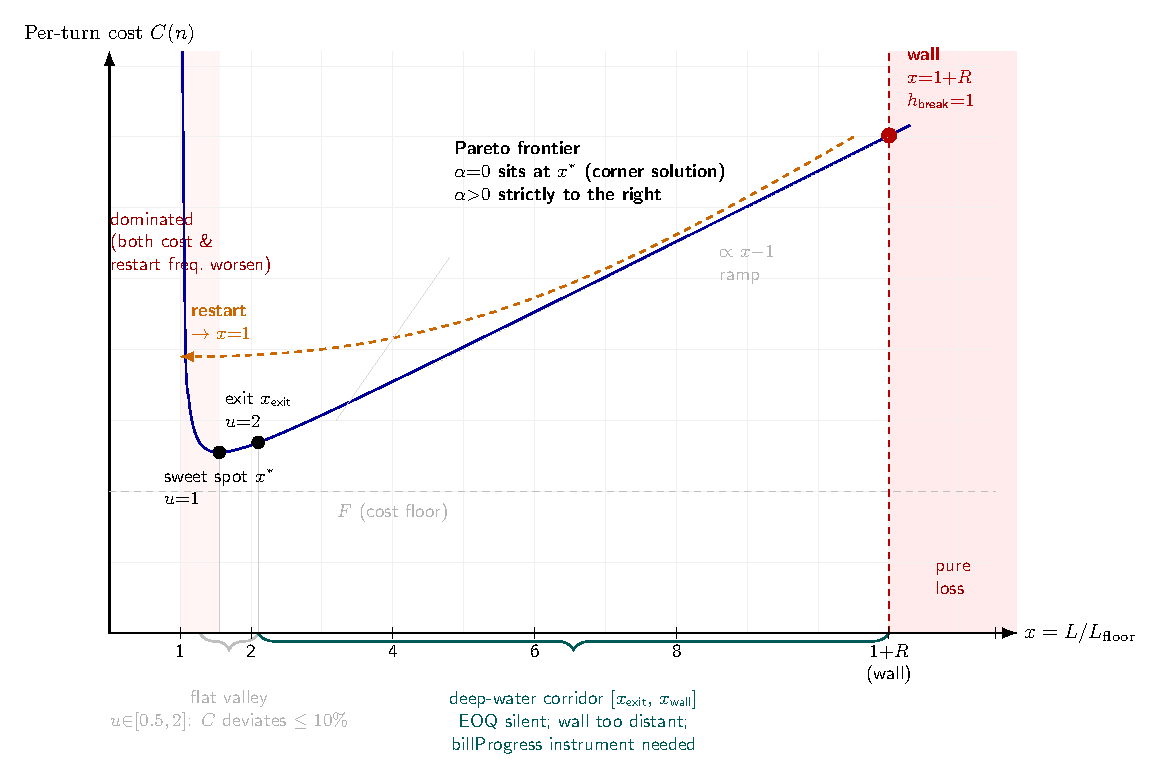
\includegraphics[width=0.92\textwidth]{fig-eoq-curve.pdf}
\caption{The EOQ cost curve for an LLM session, annotated with the structural landmarks introduced in Section~3. The U-curve plots per-turn cost $C(n)$ against normalized context length $x = L/L_{\text{floor}}$. The \textbf{sweet spot} ($u{=}1$, $x^*$) minimizes cost; to its left ($x \in [1, x^*)$), all points are Pareto-dominated (both cost and restart frequency can be improved simultaneously). From $x^*$ to the \textbf{exit line} ($u{=}2$, $x_{\text{exit}}$), the cost curve remains in the flat valley ($k \in [0.5,2]$), now on the Pareto frontier: the cost trade-off is at most 5--10\%, which is why the model stays silent there. The \textbf{wall} ($x = 1+R$) is where one more turn costs as much as a complete restart ($h_{\text{break}}{=}1$). The \textbf{deep-water corridor} between exit line and wall is the portion of the Pareto frontier where the cost trade-off becomes first-order and EOQ is silent, requiring continuous instrumentation (Section~4). A restart resets $x$ to $1$ (dashed orange arrow).}
\label{fig:eoq}
\end{figure}

The gap between exit line and wall---the ``deep-water corridor''---widens near-linearly with $R$. The structural scaling ($\propto\sqrt{R}$ for the exit offset, $\propto R$ for the wall) is general; the absolute token counts below are illustrative for one operator's setup ($L_{\text{floor}} \approx 55$K, $\kappa \approx 640$). At $R = 12.5$ (the operator's Anthropic tier), the corridor spans $\sim$114k to $\sim$743k tokens; at $R = 120$ (DeepSeek V4 Pro), it stretches from $\sim$239k to $\sim$6.7M.

The exit line and the wall thus delineate two regimes with qualitatively different guarantees. In the \textbf{flat valley} ($k \in [0.5, 2]$ around the sweet spot, $u \in [0.5, 2]$), the cost curve is nearly horizontal: timing imprecision costs at most 5--10\%, so the model's message is ``don't bother optimizing.'' In the \textbf{deep-water corridor} ($x \in [x_{\text{exit}}, x_{\text{wall}}]$, $u > 2$), EOQ is silent---the decision has moved past the optimum and the wall is too distant to be actionable---but the model is not silent: the operator's private $\alpha$ translates to an augmented buy cost (Section~\ref{sec:skirental}), shifting the effective restart trigger rightward, and every further turn of delay is a revealed preference for continuity over cost. The model's guarantee shifts from ``timing doesn't matter'' to ``you can measure what continuity is costing you''---an obligation fulfilled by the $\text{billProgress}$ gauge (Remark~\ref{rem:weld}) and the revealed-$\alpha$ inversion (Section~\ref{sec:pareto}).

\begin{remark}[The weld: burnRate as common axis]
\label{rem:weld}
The EOQ model speaks in \emph{position} language ($n^*$, $x$, exit line): it answers ``where should I restart?'' The ski-rental model speaks in \emph{rate} language ($h_{\text{break}}$, cumulative rent): it answers ``how fast am I burning?'' These are not two independent insights. A single variable collapses them:
\[
\text{burnRate} = \frac{x-1}{R} = \frac{1}{h_{\text{break}}}.
\]
The first equality is the EOQ position expressed as a rate; the second equality is the ski-rental break-even horizon recast as a burn speed. The two classical models---one from 1913, one from 1990---share a common axis in the LLM session domain, and that axis is the per-turn fraction of the rebuild cost currently being burned in avoidable rent. Every structural quantity in this paper ($n^*$, $x^*$, the 41.4\% bound, the regret function, $\text{billProgress} = u^2$) is a different projection of this single variable.
\end{remark}

\begin{remark}[Billing gauge meets inventory model]
A derived identity connects the continuous instrumentation back to the EOQ foundation. Define normalized distance from restart $u = (x-1)/\Delta$ where $\Delta = \sqrt{2\gamma}$ and $\gamma = R g / L_{\text{floor}}$. The cumulative avoidable rent burned from restart to position $u$ is $\text{billProgress}(u) = u^2$ (derivation: cumulative avoidable rent $= \int_0^t C_h g \tau \,d\tau = C_h g t^2/2 = C_h (L-L_{\text{floor}})^2/(2g)$; normalizing by the rebuild cost $C_m L_{\text{floor}}$ and substituting $u = (x-1)/\Delta$ yields $u^2$), with one ``full bill'' ($\text{billProgress}=1$) corresponding to $u=1$---the EOQ sweet spot, where the cumulative avoidable rent since the last restart equals one restart's worth of rent ($C_m L_{\text{floor}}$); this is the ski-rental break-even threshold at which continuing and restarting are cost-neutral, which is asymptotically equivalent to the optimal restart interval $n^*$. The wall ($u_{\text{wall}} = R/\sqrt{2\gamma}$) is the point where the next turn's avoidable rent equals one complete restart cost ($h_{\text{break}} = 1$); $\text{billProgress}$ there equals $R^2/(2\gamma)$. The exit line ($u=2$) corresponds to $\text{billProgress}=4$---four full restart-equivalents burned since the last restart. The billing gauge and the inventory model share a single axis; the instrument panel reports dollar burn, but every tick mark on it is a point on the EOQ U-curve.
\end{remark}

% ======================================================================
\section{Preliminary Data Collection}
% ======================================================================

We report preliminary empirical measurements from real LLM session transcripts, collected as part of an ongoing data-collection effort. All data are from a single operator (the author) across multiple providers and workflows. The measurements are not a validation of the model---cross-operator and out-of-sample data are not yet available---but they demonstrate that the model's structural quantities are observable in real billing telemetry and that the theoretical landmarks ($L_{\text{floor}}$, $g$, $R_{\text{eff}}$, $x_{\text{wall}}$) can be estimated from client-side instrumentation alone. Specific parameter values reflect one operator's workload distribution and should not be taken as universal constants.

The empirical quantities in this section fall into three categories, and the distinction matters for generalization claims:

\begin{center}
\small
\begin{tabular}{@{}l p{5.5cm} p{5cm}@{}}
\toprule
Category & Examples & Status \\
\midrule
\textbf{Structural identities} & $R_{\text{eff}}$ (Eq.~\ref{eq:reff}), $41.4\%$ bound, regret function & General---derivable from the model alone \\
\textbf{Measurable, environment-bound} & $p_{\text{ttl}} \approx 0.13$, $\rho \approx 0.07$, $L_{\text{floor}} \approx 55$K & General in form; local in value---re-measurable per operator \\
\textbf{Calibration knobs} & $N = 15$--$20\times k_{\text{stable}}$ (tooth-pitch), confirmation window & Tuning parameters---operator-specific, supplied as a template \\
\bottomrule
\end{tabular}
\end{center}

This taxonomy is the measurement philosophy of the paper: report structural results as theorems, report environment-bound quantities with their causal identity (so they can be re-measured), and report calibration knobs as recipes (so they can be re-tuned).

\subsection{Context Accumulation Linearity}

The foundational assumption of the cost model is that cumulative context length $L(t)$ grows approximately linearly with turn count. Linearity was initially observed on four controlled Playwright debugging sessions ($n = 790$--$1024$ turns; $R^2 \ge 0.957$, slope $220 \pm 30$ tok/turn, per-turn $g$ CV 2.7--8.3). We subsequently observed the same pattern on a cross-workflow corpus of 1,016 DeepSeek session transcripts from the same operator, spanning diverse coding tasks beyond debugging. Of the 1,016 transcripts, 813 were subagent side-chains (excluded from the agent-tier analysis) and 44 main transcripts contained no billable usage, leaving 159 main-session transcripts across 151 sessions. Segmentation on context-stock drop boundaries yielded 272 segments of at least 15 raw calls each; requiring at least 8 post-warmup (post-knee) positive-growth deltas dropped 17 segments, giving the 255 valid segments analyzed (238 V4-Pro, 17 V4-Flash).

Across these 255 valid segments, the median whole-segment $R^2 = 0.975$ (length-weighted mean 0.974, p10 0.905, p90 0.993). Three findings carry over from the pilot. First, cumulative $L$ is strikingly linear across workflows, not merely within the controlled Playwright setting. Second, per-turn growth $g$ fluctuates violently (CV 2.7--8.3 in the pilot; the full corpus exhibits comparable or higher dispersion) yet this volatility is absorbed at the cumulative layer---linearity lives in the integral, not the derivative. Third, at finer granularity the $L(t)$ curve exhibits a consistent plateau-and-break structure (Figure~\ref{fig:plateau-exemplars}): near-pure linear plateaus separated by discrete fold-jump injections (\S\ref{sec:foldjump}). The EOQ assumption holds on the cumulative scale---the weighted-average growth rate across segments is what feeds $g$ in Eq.~\ref{eq:growth}---even though it fails on both the per-turn and per-segment scales.

To quantify within-segment linearity, we remove fold-jump steps (\S\ref{sec:foldjump}) and compute $R^2$ on the remaining plateaus. Using the $N=15\times k_{\text{stable}}$ threshold (chosen from the pitch-scan calibration in \S\ref{sec:foldjump}; estimated pre-confirmation exceedance rate $\approx 1.4\%$ at this setting), we obtain 349 plateaus of at least 20 consecutive turns (from the same 255 segments). The length-weighted mean plateau $R^2 = 0.980$ (median 0.980, p10 0.937, p90 0.994), compared to 0.974 for whole segments. The improvement is modest ($\Delta R^2 \approx 0.006$), consistent with the fact that even whole-segment $R^2$ is already high; fold-jumps are rare within any given plateau. The direction of the gap confirms that residual nonlinearity is concentrated in discrete jump events, while the plateaus between jumps exhibit near-pure linear growth. Plateau slope varies by workflow type (median 644 tok/turn, p25--p75: 532--871), considerably higher than the Playwright pilot sessions (220 tok/turn)---an observation consistent with heavier tool-use density in general coding sessions, though the causal attribution (workflow type vs.\ model used vs.\ operator habit) has not been isolated. The structural invariant is the linear form $L(t) = L_0 + k_{\text{stable}} \cdot t$, not the specific slope value.

\begin{figure}[ht]
\centering
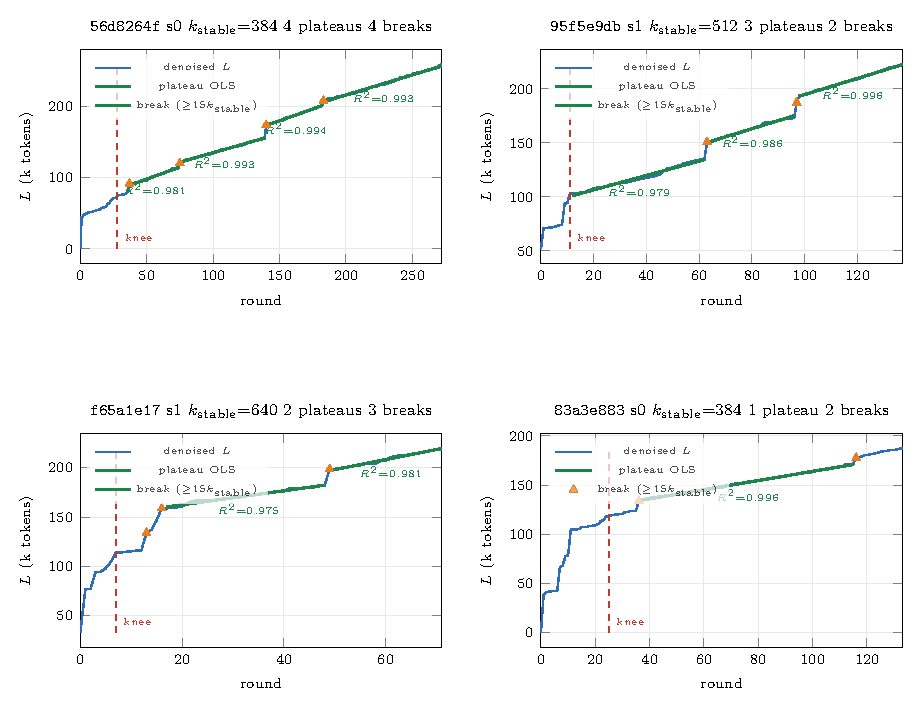
\includegraphics[width=\textwidth]{fig-plateau-exemplars.pdf}
\caption{Four representative session segments from the cross-workflow corpus, showing the plateau-and-break structure across diverse workflows and $k_{\text{stable}}$ values. Denoised context length $L(t)$ (blue) is decomposed into plateaus separated by fold-jump breaks (orange triangles, $\ge 15\times k_{\text{stable}}$). Each plateau is independently fit with OLS (green); the per-plateau $R^2$ values (0.975--0.996 across the ten plateaus shown) confirm that linearity is a within-plateau property, not merely a cumulative artifact of the integrated $L(t)$ series. The knee marker (red dashed) indicates the end of the warmup phase. Panels vary in plateau count (1--4) and stable growth rate $k_{\text{stable}}$ (384--640 tok/turn), illustrating the structural invariance of the linear form $L(t)=L_0+k_{\text{stable}}\cdot t$ across workflow types.}
\label{fig:plateau-exemplars}
\end{figure}

A methodological note: $L(t) = \sum_{\tau=1}^t g(\tau)$ is an integrated ($I(1)$) process. For any stationary $g$ with positive mean, $R^2$ of $L(t) \sim t$ converges mechanically toward 1 as $t$ grows \citep{granger1974}. To assess the severity of this concern, we run two diagnostics on the $g(t)$ series across the 255 valid segments. First, an augmented Dickey-Fuller (ADF) test on $L(t)$: median test statistic $t = -2.04$, with 65\% of segments failing to reject the unit-root null at the 5\% level---confirming that $L(t)$ is indeed $I(1)$ and that $R^2$ values must be interpreted with this in mind. Second, the same test on $g(t) = \Delta L(t)$: median $t = -10.92$, with 100\% rejecting the unit-root null---so the per-turn growth rate $g(t)$ is stationary. A Ljung-Box $Q(10)$ test on $g(t)$ yields median $Q = 7.4$, with only 16\% of segments exhibiting significant autocorrelation. To quantify the mechanical contribution of integration to $R^2$: a permutation null that shuffles per-turn increments $g(t)$ within each segment (preserving their empirical distribution but destroying any genuine trend structure) produces a median whole-segment $R^2 = 0.937$, close to the observed 0.975---confirming that $R^2$ of $L(t) \sim t$ is largely a consequence of $I(1)$ integration rather than an independent measure of linearity. The primary, non-cumulative evidence for linear structure is therefore the stationarity of $g(t)$ (100\% unit-root rejection) and the cross-plateau consistency of $k_{\text{stable}}$ (p25--p75: 532--871 tok/turn, depending on workflow density). The residual autocorrelation (16\% of segments) is concentrated at fold-jump boundaries, consistent with the plateau-and-break structure.

This corpus is the same DeepSeek dataset underlying the reconstruction in Section~4.2.1, viewed through a different filter chain. The 151 sessions here correspond to the 160 sessions of Section~4.2.1 (the 9-session gap is accounted for by the reconstruction's independent folding and tiering filters). Within the 255 segments, fold-jump removal produces 349 plateaus of at least 20 consecutive turns; these plateaus, not the raw segments, are the units on which per-plateau $R^2$ and $k_{\text{stable}}$ are computed. The reconstruction pipeline (Section~4.2.1) operates on the same underlying month of DeepSeek V4 billing (June 2026), yielding 42,697 folded API calls after message.id deduplication, of which 145 agent-tier sessions had $n \ge 5$ and $g > 0$.

\subsection{Effective Cost Ratio in Practice}

The nominal cost ratio $R$ in Table~\ref{tab:providers} is a provider-published constant. In practice, the \emph{effective} cost ratio $R_{\text{eff}}$ deviates from $R$ for at least two structural reasons beyond per-turn workload variation. Both are captured by the same formalism---$R_{\text{eff}} = R / q$ where $q \ge 1$ is an inflation factor---but arise from distinct provider-side mechanisms.

\subsubsection{Forward Bill Reconstruction}

We assess the model by reconstructing provider billing from per-turn session logs---a \emph{forward} direction that breaks the circularity of inferring both $g$ and $L_{\text{avg}}$ from the same billing aggregate. The reconstruction is a structural decomposition exercise, not a predictive model: it demonstrates that the model's three-way split (holding, order, output) maps onto separable line items in real provider invoices and can be recovered from client-side telemetry alone. The 91\% recovery figure is an existence proof that the decomposition is observable, not a model-selection score. The reconstruction pipeline ingests washed per-API-call usage records (content-free; only token counts and model tier retained, folded by message.id to eliminate streaming-snapshot double-counting), applies three deterministic rules, and produces a daily predicted bill that is compared against the raw provider invoice.

The three reconstruction rules were developed through iterative reconciliation against a single month of DeepSeek V4 billing (June 2026, 160 sessions, 42,697 folded calls). The evaluation window begins June~9 because JSONL transcript export---the input to the reconstruction pipeline---was not deployed until that date; the billing record extends back to June~3 but the corresponding transcripts are unavailable, so June~3--8 are excluded from the reconciliation window.\footnote{Because the rules were fit and evaluated on the same billing month, the 91\% recovery is \emph{in-sample}. A held-out period or second provider/operator would be needed to estimate out-of-sample generalization; neither is available in this study.}:

\begin{enumerate}[leftmargin=*,itemsep=0pt,topsep=0pt]
\item \textbf{message.id folding.} A single API call emits multiple usage-bearing streaming snapshots with identical \texttt{cache\_read}. Folding to the last snapshot per message.id removes 58\% of raw rows and brings the total to the correct order of magnitude; without it, accumulated context stock is overestimated by $\sim$2.4$\times$.
\item \textbf{Tier by model, matching the bill.} The provider invoice separates billing lines by model tier (e.g., \texttt{deepseek-v4-pro} vs.\ \texttt{deepseek-v4-flash}). The reconstruction must tier by model, not by the transcript's \texttt{isSidechain} flag: a main session can contain inline flash-model calls that belong to the flash bill line, not the agent line. Tiering by \texttt{isSidechain} produced a spurious 2.72$\times$ miss ratio on one day; tiering by model recovers the correct 0.82$\times$.
\item \textbf{Per-turn miss = input\_tokens.} Cache-miss is billed on \emph{every} turn's uncached input, not only on cold-start turns. In this DeepSeek corpus \texttt{cache\_creation} $\equiv 0$, so $\text{miss} \equiv \text{input\_tokens}$. The earlier cold-start-only assumption gave 0.33$\times$ on the miss component; per-turn accounting recovers 0.91$\times$.
\end{enumerate}

Field-to-bill mapping: $\text{cache-hit} \leftarrow \text{cache\_read}$, $\text{cache-miss} \leftarrow \text{cache\_creation} + \text{input\_tokens}$, $\text{output} \leftarrow \text{output\_tokens}$. Provider prices ($C_{\text{miss}}/C_{\text{hit}} = 120\times$ for the pro tier, $50\times$ for flash) are read from the invoice itself, not assumed.

\begin{table}[ht]
\centering
\caption{Forward bill reconstruction: per-component ratios and dollar error. Ratios are reconstruction/bill; 1.0 = perfect. Twenty days, June 9--28, 2026. Full daily table in the accompanying data package.}
\label{tab:recon}
\begin{tabular}{l c c c}
\toprule
Component & Median & Mean & Range \\
\midrule
Cache-hit (holding, $\Sigma L$) & 0.87$\times$ & 0.87$\times$ & 0.78--0.94$\times$ \\
Cache-miss (order, per-turn input) & 0.91$\times$ & 0.90$\times$ & 0.73--1.02$\times$ \\
Output tokens & 0.98$\times$ & 0.97$\times$ & 0.92--1.00$\times$ \\
\midrule
\textbf{Dollar total} & \textbf{0.91$\times$} & \textbf{0.91$\times$} & \textbf{0.82--0.97$\times$} \\
\bottomrule
\end{tabular}
\end{table}

Table~\ref{tab:recon} summarizes the reconstruction. The pipeline recovers a median 91\% of the billed dollar amount (bootstrap 95\% CI: [0.895, 0.924], 10,000 resamples across the 20 clean days; aggregate $\Sigma$R$/\Sigma$B = 0.907, 95\% CI [0.887, 0.925]), with all three cost components aligned to their respective bill lines. The output component recovers near-perfectly (0.98$\times$); the cache-hit component (holding, integrating $\Sigma L(t)$ across turns) recovers 0.87$\times$; the cache-miss component (order, per-turn uncached input) recovers 0.91$\times$. The 9\% systematic underestimate is a \emph{coverage} gap---some calls are not captured in the exported transcripts---not a pricing-rule error (a pricing error would shift one component, not all three in proportion). The reconstruction reads input and output as separate fields at their own prices, avoiding the merged-$g$ simplification of Eq.~\ref{eq:growth} for validation purposes.

Two naive baselines bound the reconstruction error. A \emph{no-cache} baseline (all context tokens priced at $C_{\text{write}}$) overestimates the bill by $\sim$53$\times$, and a \emph{cold-start-only} baseline (all context tokens priced at $C_{\text{read}}$) underestimates it to 0.59$\times$ (41\% low). The 91\% reconstruction sits between these extremes because it correctly separates the 99\% of context tokens served from cache (at $C_{\text{read}}$) from the 1\% uncached (at $C_{\text{write}}$). The no-cache baseline's 53$\times$ error is a direct consequence of mispricing cache-hit tokens at the cache-write rate ($R=120$): the three-way decomposition is not a marginal improvement over a simpler estimator---it is the structural minimum required to bring the error below an order of magnitude.

% ---- Temporal hold-out split of the reconstruction (addresses in-sample concern) ----
To address the concern that the 91\% recovery reflects in-sample tuning, we freeze the reconstruction rule set (R1--R3 and the per-tier prices, all taken from the bill) on the first 15 clean days and apply it \emph{unchanged} to the held-out final 5 days. The reconstruction has no fitted continuous parameters---the three rules are structural (message-\texttt{id} folding, subagent exclusion, per-turn miss) and the unit prices are read from the invoice---so this split tests \emph{rule stability across time}, not parameter extrapolation. Table~\ref{tab:tempsplit} shows the held-out error does not degrade: the held-out aggregate $\Sigma$R$/\Sigma$B $= 0.927$ slightly exceeds the calibration window's $0.901$, and per-component the held-out medians are $0.90\times$ (hit), $0.95\times$ (miss), $0.96\times$ (output). This rules out the interpretation that the rules were quietly fit to the evaluation days; it does \emph{not} establish cross-operator or cross-month generalization, which remains untested (\S\ref{sec:limitations}).

\begin{table}[ht]
\centering
\caption{Temporal hold-out of the forward reconstruction. Rules and prices are frozen on the calibration window and applied unchanged to the held-out days. Ratios are reconstruction/bill (1.0 = perfect). ``Aggregate'' is $\Sigma_{\text{days}}\text{recon}/\Sigma_{\text{days}}\text{bill}$. Same single operator and billing month throughout---this is a within-month stability check, not out-of-sample validation.}
\label{tab:tempsplit}
\begin{tabular}{l c c c c}
\toprule
Window & Days & Median & Aggregate $\Sigma$R$/\Sigma$B & Range \\
\midrule
Calibration (Jun 9--23) & 15 & 0.905 & 0.901 & 0.821--0.956 \\
Held-out (Jun 24--28)   & 5  & 0.931 & 0.927 & 0.827--0.966 \\
\midrule
All clean days          & 20 & 0.912 & 0.907 & 0.821--0.966 \\
\bottomrule
\end{tabular}
\end{table}

The reconstruction scripts, the washed usage table, and the daily reconciliation output are included in the repository so that reviewers can reproduce the result.

\begin{remark}[Operator restart discipline]
The forward reconstruction demonstrates the fit of the cost model's \emph{structure}---the three-way decomposition into holding, order, and output---on this operator's billing month, with the in-sample caveat noted above. The operator's \emph{behavior} is measured separately from the billing aggregates. Across 145 agent-tier sessions ($n \ge 5$, $g > 0$) in the same billing month, the session length relative to the EOQ optimum---$k = n / n^*$, where $n$ is the observed turn count and $n^* = \sqrt{2 R L_{\text{floor}} / g}$ is computed per-session from its fitted $L_{\text{floor}}$ and $g$---distributes as: median $1.8$, p25--p75 $1.1$--$2.4$, tail ($k > 3$) 14\%. The median session runs roughly $1.8\times$ longer than the cost-minimizing length, and 82\% of sessions exceed their per-session $h_{\text{break}}$ (warm-reuse is cheaper than a fresh restart). Because the cost curve is flat near the optimum (Section~\ref{sec:sensitivity}, $k \in [0.5, 2]$ costs at most 5--10\% above the minimum), the median session sits inside the flat valley despite the deviation. The model's primary value is not in shaving the last few percent off a near-optimal operator, but in identifying the 14\% tail ($k > 3$) where unbounded regret materializes.
\end{remark}

\subsubsection{Cold-Start Rebuild: When the Floor Is Not Cached}

A systematic discrepancy exists between the model's idealized restart cost and observed billing telemetry. Equation~\eqref{eq:nstar} prices the rebuild floor $L_{\text{floor}}$ at $C_m$ (write) rates---the worst-case assumption $p_{\text{cold}}=1$, i.e., every token of the floor is a cold write, and a fresh session pays the full rebuild cost. This is conservative: in practice, some fraction of the floor may be byte-identical across sessions and eligible for cache reuse. But turn~0 of a restarted session frequently records $\text{cache\_read} \approx 0$, billing the entire $L_{\text{floor}}$ at $C_{\text{write}}$ rates, confirming that the worst-case assumption is often realized. The measured probability of full write, denoted $p_{\text{cold}}$, interpolates between the fully warm floor ($p_{\text{cold}}=0$, all tokens hit cache at $C_{\text{read}}$) and the Eq.~\eqref{eq:nstar} worst case ($p_{\text{cold}}=1$, all tokens billed at $C_{\text{write}}$). The effective rebuild cost is $C_m L_{\text{floor}} p_{\text{cold}} + C_h L_{\text{floor}} (1-p_{\text{cold}})$, and the effective optimum is $n^*_{\text{eff}} = n^* \cdot \sqrt{(1+(R-1)p_{\text{cold}})/R}$ (Section~\ref{sec:cost-decomposition}). For the measured values (Claude: $p_{\text{cold}} \approx 0.72$, $R=12.5$, $n^*_{\text{eff}}/n^* \approx 0.86$; DeepSeek: $p_{\text{cold}} \approx 0.97$, $R=120$, $n^*_{\text{eff}}/n^* \approx 0.99$), the correction is modest and conservative---the nominal $n^*$ overestimates the cost-minimizing interval by at most $\sim$14\%, well within the flat valley---so the model's restart recommendation is slightly late in pure dollar terms, a bias that the guardrail interpretation accepts.

The mechanism has two components. The primary cause is provider-side session isolation: different session IDs do not share cached prefixes even when the byte content is identical. The secondary cause is TTL expiry during inter-session idle gaps. The two mechanisms are distinguished by their observable signatures: session-ID isolation produces near-zero turn-0 cache hits on every fresh session regardless of idle duration; TTL expiry produces a hit-rate gradient with idle time.

% ---- Idle-gap gradient: separates session-ID isolation from TTL expiry ----
We separate the two mechanisms empirically by binning each cold start on the idle gap since the prior session's last activity in the same project directory. Session-ID isolation predicts an idle-independent floor of zero-hit restarts; TTL expiry predicts a hit-rate gradient that decays with idle time. Both signatures are present (Table~\ref{tab:idlegrad}): turn-0 hit declines monotonically from $0.34$ (under 1~min) to $\approx 0.09$ beyond 5~min---the TTL signature---while even sub-TTL restarts retain a $56\%$ zero-hit floor---the isolation signature that no idle-time reduction removes. Aggregated, restarts with $<5$~min idle show $56\%$ zero-hit (mean hit $0.26$) versus $81\%$ zero-hit (mean hit $0.09$) beyond 5~min, consistent with Anthropic's 5-minute default TTL superimposed on unconditional session-ID isolation. The sample is small ($n=35$ restarts with a measurable prior-session gap, from 69 true cold starts after subagent exclusion); the gradient is suggestive of the two-mechanism decomposition rather than a precise rate estimate.

\begin{table}[ht]
\centering
\caption{Claude turn-0 cache hit vs.\ idle gap since the prior same-project session. The monotone decay is the TTL-expiry signature; the nonzero zero-hit fraction at $<5$~min idle is the session-ID-isolation floor. Single operator, $n=35$ gapped restarts (Anthropic, 5-min default TTL); bins with $n\le3$ are shown for completeness but are individually noisy.}
\label{tab:idlegrad}
\begin{tabular}{l c c c}
\toprule
Idle gap & $n$ & Zero-hit \% & Mean turn-0 hit \\
\midrule
$<1$ min      & 3 & 33 & 0.34 \\
1--5 min      & 6 & 67 & 0.22 \\
5--30 min     & 7 & 86 & 0.05 \\
30--60 min    & 5 & 80 & 0.12 \\
$>6$ h        & 9 & 78 & 0.11 \\
\midrule
$<5$ min (TTL alive)   & 9  & 56 & 0.26 \\
$\ge 5$ min (TTL expired) & 26 & 81 & 0.09 \\
\bottomrule
\end{tabular}
\end{table}

Measured across 69 Claude true cold starts (Anthropic, 5-min TTL, after excluding subagent transcripts---a subagent's first call inherits the parent's task context and spuriously appears warm), 72\% recorded zero cache reads on turn~0. Across 158 DeepSeek true cold starts, 97\% recorded zero cache reads. Both figures use the same measurement discipline (main-session cold starts only). The two providers are materially different---$p_{\text{cold}}$ is provider-dependent, not a universal constant---and the gap (0.72 vs.\ 0.97) reflects the different TTL regimes: DeepSeek's hours-to-days TTL makes intra-session cache irrelevant to inter-session cold starts, while Anthropic's 5-minute TTL occasionally leaves residual system-prefix cache alive across a restart.

Relative to a hypothetical fully warm floor (all tokens at $C_{\text{read}}$), the cold-start miss raises the effective rebuild cost above the read-price ideal. Let $p_{\text{cold}}$ denote the probability that a restart incurs a full write on $L_{\text{floor}}$, estimated as the fraction of true cold-start sessions recording zero turn-0 cache reads (using the same measurement discipline described above). The measurements give $p_{\text{cold}} \approx 0.72$ for Claude ($N = 69$, 5-min TTL) and $p_{\text{cold}} \approx 0.97$ for DeepSeek ($N = 158$). The Claude figure means roughly one restart in four recovers a partial system-prefix cache hit, while the DeepSeek floor is near-fully rewritten on essentially every restart. The effective rebuild cost is $C_m \cdot L_{\text{floor}} \cdot p_{\text{cold}} + C_h \cdot L_{\text{floor}} \cdot (1-p_{\text{cold}})$; for the author's coding environment ($L_{\text{floor}} \approx 55$K tokens, $R = 12.5$, $p_{\text{cold}} \approx 0.72$), this adds $\sim$$C_m \cdot 40\text{K}$ per restart in expectation. The structural point---that a cold-start miss bills byte-identical prefixes at write rates---holds for any provider that isolates cache across sessions, but the severity is provider-dependent. The two mechanisms have different policy implications: TTL-induced cold starts can be mitigated by faster dispatch loops; session-ID isolation cannot be mitigated by any client-side action.

The forward reconstruction uses \emph{actual} restart costs from telemetry, not the model's worst-case assumption.

\subsubsection{TTL-Induced Collapse in Orchestrator Workflows}
\label{sec:ttl}

In orchestrator sessions where a parent agent dispatches subagents, the parent's context goes idle during subagent execution. If the idle gap exceeds the provider's cache TTL (5~minutes for Anthropic's default tier), the re-entry turn rewrites the parent context at cache-write rates, collapsing $R_{\text{eff}}$.

Let $p_{\text{ttl}}$ denote the fraction of dispatches whose duration exceeds the TTL. The effective read cost becomes a weighted average of warm hits (at $C_{\text{read}}$) and cold misses (at $C_{\text{write}}$):

\begin{equation}
\bar{C}_{\text{read}} = (1-p_{\text{ttl}}) \cdot C_{\text{read}} + p_{\text{ttl}} \cdot \bigl[\rho \cdot C_{\text{read}} + (1-\rho) \cdot C_{\text{write}}\bigr]
\quad\Longrightarrow\quad
R_{\text{eff}} = \frac{C_{\text{write}}}{\bar{C}_{\text{read}}} = \frac{R}{1 + p_{\text{ttl}} \cdot (1-\rho) \cdot (R-1)}
\label{eq:reff}
\end{equation}

where $\rho$ is the fraction of parent stock that survives the miss as system-prefix cache hits (measured $\rho \approx 0.07$--$0.10$).

We measure $p_{\text{ttl}}$ from five Claude orchestrator sessions (Anthropic, 5-min TTL; 236 dispatches total, pooled $p_{\text{ttl}} = 0.20$) and 17 DeepSeek counterfactual sessions ($n = 403$ dispatches, pooled $\hat{p}_{\text{ttl}} = 0.02$). The $\sim$10$\times$ gap (0.20 vs.\ 0.02) mirrors the TTL asymmetry: Claude's 5-min TTL makes orchestrator sessions routinely exceed the cache lifetime, while DeepSeek's long TTL keeps most re-entries warm. Per-session $p_{\text{ttl}}$ ranges from 0.02 (a session with no long dispatches) to 0.59 (a session where 12 of 22 dispatches exceeded 5~minutes), reflecting strong dependence on dispatch density rather than a single universal rate. Table~\ref{tab:ttl} shows the impact of a representative $p_{\text{ttl}} = 0.26$ on $R_{\text{eff}}$.

\begin{table}[ht]
\centering
\caption{TTL-induced $R_{\text{eff}}$ collapse and downstream effects (merge $p_{\text{ttl}} = 0.26$, $\rho \approx 0.07$).}
\label{tab:ttl}
\begin{tabular}{lcc}
\toprule
Metric & Nominal ($R = 12.5$) & Effective ($R_{\text{eff}} \approx 3.4$) \\
\midrule
Cost ratio & $12.5$ & $\approx 3.4$ \\
burnRate $(x-1)/R$ (at $x = 2$) & $0.08$ & $\approx 0.29$ ($\times 3.7$) \\
$h_{\text{break}}$ (at $x = 2$) & $\approx 12.5$ turns & $\approx 3.4$ turns \\
EOQ exit offset $\propto \sqrt{R}$ & baseline & $\approx 0.52\times$ \\
\bottomrule
\end{tabular}
\end{table}

The 5-minute cliff is sharp: dispatches exceeding 5~minutes show $100\%$ miss rate across both independently measured Anthropic sessions; dispatches under 5~minutes show $0$--$7\%$ miss rate (the residual $\approx 7\%$ is attributable to provider-side eviction or prefix drift). The structural identity $R_{\text{eff}} = R / (1 + p_{\text{ttl}}(1-\rho)(R-1))$ is the general takeaway; the specific $p_{\text{ttl}}$ value is workload-dependent.

\subsubsection{Separation of Concerns}

The cold-start miss and the TTL collapse affect different terms in the cost function and do not combine into a single scalar inflation factor. The cold-start miss governs the \emph{order} term: Eq.~\eqref{eq:nstar} prices the rebuild floor at $C_m \cdot L_{\text{floor}}$ (the $p_{\text{cold}}=1$ worst case), while the empirical effective rebuild cost is the expectation $C_m \cdot L_{\text{floor}} \cdot p_{\text{cold}} + C_h \cdot L_{\text{floor}} \cdot (1-p_{\text{cold}})$. Since $p_{\text{cold}} \le 1$, the effective order cost never exceeds the model's conservative assumption; the $n^*_{\text{eff}}$ correction derived in Section~\ref{sec:ttl} quantifies this modest downward adjustment. The TTL collapse inflates the \emph{holding} term: the per-turn read price $C_{\text{read}}$ is replaced by the effective $\bar{C}_{\text{read}}$ from Eq.~\ref{eq:reff}, yielding $R_{\text{eff}}$ as derived in Section~\ref{sec:ttl}. Because the two mechanisms act on different cost components (one-time restart vs.\ per-turn read), collapsing them into a single $R_{\text{eff}}$ would conflate a quantity that governs the rebuild decision with one that governs the holding rate. The cost model keeps them separate: the rebuild cost is provider-measured and entered as a parameter; the holding rate uses $R_{\text{eff}}$ from Eq.~\ref{eq:reff}. Both are measurable from client-side telemetry without provider-side instrumentation.

\subsection{Fold-Jump Detection and the Upward Regeneration Point}
\label{sec:foldjump}

In tool-heavy agentic loops, context grows not smoothly but in discrete ``fold jumps''---large one-time injections such as loading a fixture file or reading a large source module. Under the renewal framework (Section~3.5), a restart is a \emph{downward} regeneration point ($L$ resets to $B_{\text{rebuild}}$). A fold-jump is its dual: an \emph{upward} regeneration point where $L$ jumps discretely without a restart, permanently raising the effective $B_{\text{rebuild}}$ for the remainder of the session.

We detect fold-jumps by tracking the residual $r(t) = L(t) - L_{\text{pred}}(t)$ where $L_{\text{pred}}$ is the linear extrapolation from the last latched baseline using a stable per-session growth rate $k_{\text{stable}}$. A fold-jump is declared when $r(t)$ exceeds $N \cdot k_{\text{stable}}$ and persists (does not revert within a confirmation window).

Calibrated on the same 1,016 DeepSeek session transcripts: 255 segments contained sufficient post-warmup data, 131 sessions (51\%) exhibited at least one fold-jump, and 1,259 total jumps were detected at the $N{=}8\times k_{\text{stable}}$ threshold. At $N{=}20\times$ (used as the provisional operational threshold) the count drops to 202 jumps across the corpus. The post-warmup $\Delta L / k_{\text{stable}}$ distribution (Figure~\ref{fig:postknee}) is monotonically decreasing with no bimodal gap (p50 $=$ 1.0$\times$, p95 $=$ 7.7$\times$, p99 $=$ 17.5$\times$), with true jumps occupying the upper tail. Tooth spacing $N \approx 15$--$20\times k_{\text{stable}}$ cleanly separates true injections from per-turn noise (estimated pre-confirmation exceedance rate $\approx$0.75\% at $N{=}20\times$). The specific $N$ value is operator- and workflow-dependent; the structural point is that no natural boundary exists in the distribution, meaning $N$ is a precision/recall knob, and persistence confirmation (the jump must \emph{hold} at the new level) is the primary discriminator between genuine injections and large transient spikes.

\begin{figure}[ht]
\centering
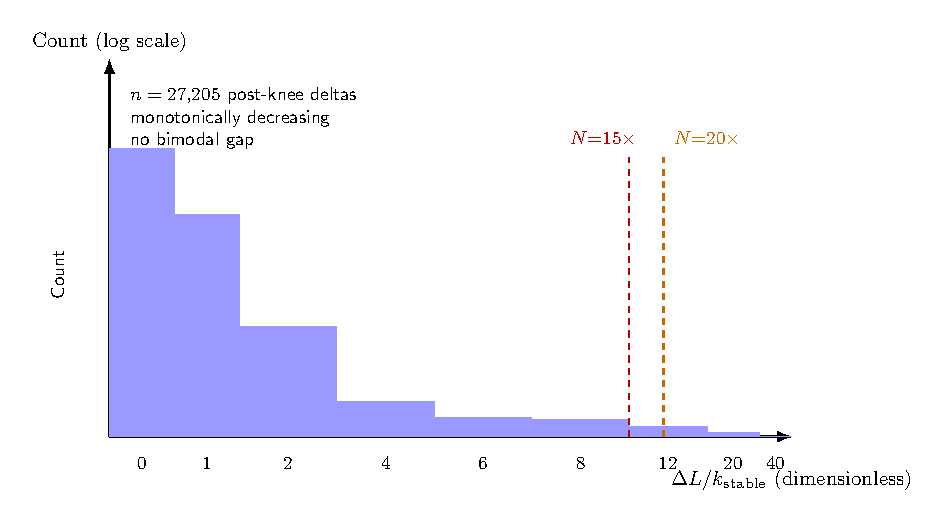
\includegraphics[width=0.85\textwidth]{fig-postknee-hist.pdf}
\caption{Distribution of post-warmup $\Delta L / k_{\text{stable}}$ across 27,205 delta observations from 1,016 session transcripts. The distribution is monotonically decreasing with no bimodal gap between ``noise'' and ``signal''---there is no natural boundary. The dashed lines mark two candidate tooth-pitch thresholds ($N{=}15\times$ and $N{=}20\times$); the choice between them is a precision/recall trade-off, not a structural distinction.}
\label{fig:postknee}
\end{figure}

The measurement layer operates without $\alpha$: it detects the step and adjusts the full-carry baseline, but never judges whether the injected mass is ``benign reusability'' or ``malignant bloat.'' That verdict remains with the human operator, who alone possesses the semantic context to classify the mass. This is the same measurement/verdict split that governs the restart decision itself.

This split is a deliberate architectural invariant, not a capability gap: automated classification of semantic mass would leak task-structure assumptions into a cost instrument (Section~6.1), and no oracle exists for $\alpha$.

% ======================================================================
\section{Discussion}
% ======================================================================

\subsection{Why the Flat Valley Liberates}

The cost model produces an initially paradoxical result: the optimum is mathematically precise ($n^*$ is a closed-form expression), yet deviating from it by a factor of 2 costs a few percent at most. The 41.4\% bound quantifies why: the floor dominates. The practical implication is that \emph{precise restart timing is not worth optimizing}. What \emph{is} worth preventing is the tail: $k \to \infty$ regret is unbounded.

This reframes the tool's value proposition. It is not a precision optimizer that extracts the last 1\% of timing efficiency from a fundamentally shallow optimum. It is cheap insurance against tail explosions---the sessions that run $n = 10n^*$ because no one noticed the context bill until it was enormous. The regret function $(k + 1/k - 2)/2 \cdot A(n^*)$ is the formal version of this intuition: it grows without bound as $k \to \infty$, regardless of how pathological the demand sequence becomes, while remaining flat near the optimum.

Critically, tail risk is not a property of the operator---it is a property of $R$. The optimal restart interval scales as $n^* \propto \sqrt{R}$ (Eq.~\ref{eq:nstar}). A session pattern that is near-optimal on a high-$R$ provider can be deep in the tail on a low-$R$ provider without any change in operator behavior. Concretely: a session of 80 turns that sits comfortably near $n^*$ on DeepSeek V4 Pro ($R \approx 120$, $n^* \approx 90$) operates at $k \approx 2.5$ on Claude ($R \approx 12.5$, $n^* \approx 32$) and at $k \approx 6.4$ on a hypothetical $R=5$ provider ($n^* \approx 12.5$). The same human, the same workflow, the same attention level---three radically different cost multiples. Tail events need not be \emph{observed} in a single-provider corpus to be \emph{structurally inevitable} under provider migration. This is not an empirical claim about a specific operator's sessions; it is a direct consequence of the square-root scaling in the EOQ optimum: halving $R$ shrinks $n^*$ by $1/\sqrt{2}$, pushing every existing session length further into the right tail. The regret function, which depends only on the deviation multiple $k$ and not on $R$ directly, catches these cases automatically: a session running at $k=6.4$ incurs $(6.4 + 1/6.4 - 2)/2 \approx 2.28\times$ the movable cost at the optimum, regardless of provider.

\begin{proposition}[Policy-level $\alpha$-free guarantees]
\label{prop:alphafree}
If the operator executes restarts at the ski-rental cumulative-rent threshold (restart when total avoidable rent since last restart reaches $C_m B_{\text{rebuild}}$), the policy provides three guarantees that do not depend on $\alpha$, which the model can neither measure nor assume:
\begin{enumerate}[leftmargin=*,itemsep=0pt,topsep=0pt]
\item \textbf{Exact regret per cycle:} deviation from the optimal interval $n^*$ by a factor $k = n/n^*$ incurs exact regret $(k + 1/k - 2)/2 \cdot A(n^*)$. The regret is convex in $k$, flat near the optimum (at most 5--10\% for $k \in [0.5, 2]$), and unbounded as $k \to \infty$;
\item \textbf{Dollar-cost wall:} when context length reaches $L_{\text{wall}} = L_{\text{floor}} \cdot (1 + R)$, continuing one more turn costs as much as a complete restart in pure dollar terms ($h_{\text{break}} = 1$). The wall position is $\alpha$-independent; the augmented wall (including $V_\alpha$) lies further right, so the dollar-cost wall provides a conservative alarm that is valid for every $\alpha \ge 0$;
\item \textbf{Restart interval bounds:} the model maps every restart decision onto the pure-dollar interval $[x^*, x_{\text{wall}}]$; the operator's private $\alpha$ determines \emph{where} in this interval, but the model's cost envelope ensures no point is left of $x^*$ (cost-dominated by restarting earlier) or right of $x_{\text{wall}}$ (cost-dominated by restarting immediately in pure dollar terms). When $V_\alpha > 0$, the augmented interval extends rightward to $x_{\text{wall}} + V_\alpha/(C_h L_{\text{floor}})$, and the operator may choose a point beyond $x_{\text{wall}}$---a revealed preference, not a cost error.
\end{enumerate}
These guarantees are properties of the restart policy, not of the passive dashboard---they activate when the operator acts on the signal, not when the signal is merely displayed. The tool is a sidecar instrument; the guarantees belong to the policy it recommends.
\end{proposition}

\subsection{The Pareto Frontier of Restart Timing}
\label{sec:pareto}

The restart decision is naturally a two-objective problem. Axis~A is dollar cost, computable from the model. Axis~B is restart frequency---or equivalently, continuity loss: each restart requires a bridging summary that is both token-expensive and fidelity-lossy. Axis~B's magnitude is governed by $\alpha$, the operator's subjective continuity valuation introduced in Section~3.6. $\alpha$ is a preference, not a prediction; the model cannot measure it and does not attempt to.

The model's pure-dollar Pareto frontier is the interval $[x^*, x_{\text{wall}}]$ where $x^* = L(n^*)/L_{\text{floor}}$ is the sweet spot (the cost-minimizing corner, $u=1$) and the exit line $x_{\text{exit}} = L_{\text{exit}}/L_{\text{floor}}$ introduced in Section~\ref{sec:twolaws} (the formal flat-valley boundary at $u=2$; Section~\ref{sec:sensitivity}) sits \emph{on} this frontier, not at its left boundary. Points to the left of $x^*$ are Pareto-dominated (both cost and restart frequency can be improved simultaneously). The frontier's left segment ($x \in [x^*, x_{\text{exit}}]$, $u \in [1, 2]$) lies within the flat valley ($k \in [0.5, 2]$): cost varies by at most 5--10\%, so the model's message is ``don't bother optimizing.'' To the right of $x_{\text{exit}}$, the Pareto trade-off between cost and continuity becomes first-order. The sweet spot $x^*$ is optimal only when continuity is valued at zero ($\alpha = 0$). Any operator with $\alpha > 0$ strictly prefers a point to the right of $x^*$; the exit line $x_{\text{exit}}$ is where that preference becomes economically measurable. The right endpoint $x_{\text{wall}} = 1+R$ is the hard cost boundary where one more turn costs as much as a complete restart; when $V_\alpha > 0$, the augmented frontier extends rightward to $x_{\text{wall}} + V_\alpha/(C_h L_{\text{floor}})$. The operator's remaining horizon $H$, compared against $h_{\text{break}}$, selects the point on this frontier.

This framing sharpens the role of $x_{\text{exit}}$. It is not ``the answer''---it is the left anchor that brackets the human choice interval. The toolbox computes the frontier; the operator, with private knowledge of $\alpha$ and $H$, picks the point.

\begin{remark}[Revealed continuity valuation]
\label{rem:revealedalpha}
Section~\ref{sec:skirental} introduced the augmented buy cost $C_m B_{\text{rebuild}} + V_\alpha$, where $V_\alpha$ is the dollar-equivalent continuity valuation. The generalized trigger condition $\sum C_h \cdot g \cdot t \ge C_m B_{\text{rebuild}} + V_\alpha$ implies that an operator who restarts at $\text{billProgress} = b$ reveals
\[
V_\alpha = (b - 1) \cdot C_m B_{\text{rebuild}}.
\]
An operator who restarts at the EOQ sweet spot ($b = 1$) reveals $V_\alpha = 0$---continuity is valued at zero, and the restart decision is pure cost minimization. An operator who delays restart to $b = 3$ reveals a continuity valuation of twice the rebuild cost: they are willing to burn two extra restart-equivalents in rent to preserve the working context. The model's Pareto frontier $[x^*, x_{\text{wall}}]$ is computed in pure dollar terms ($V_\alpha = 0$); the augmented frontier extends rightward to $x_{\text{wall}} + V_\alpha/(C_h L_{\text{floor}})$. Since $V_\alpha \ge 0$, the pure-dollar wall is a conservative inner bound, and the operator's restart point sweeps out an $\alpha$-indexed family of trigger thresholds anchored at $[x^*, x_{\text{wall}}]$ and extending beyond as $V_\alpha$ grows.
\end{remark}

\subsection{Inter-Session Dispatch}

The model's full decision scope extends beyond the single-session restart decision. An \textbf{inter-session} decision-maker---an entity that owns the lifecycle of multiple sessions---faces the question: ``should the next task reuse an existing warm session, or spawn a fresh one?'' The cost terms are identical (rebuild cost vs.\ cumulative rent), but the decision variable shifts from $n$ (turns in this session) to the session-to-task assignment policy.

The following is a design implication of the cost model, not an evaluated system (we have no orchestrator-level data). The natural home for this decision is the emerging class of LLM task orchestration platforms (Google ADK, Substrate, oh-my-claudecode, Azure Durable Task, MOCO, and others). These platforms currently make session-reuse decisions via engineering heuristics: subagents always receive fresh context windows, compaction triggers at a fixed token-budget threshold, and checkpoint intervals are chosen by convention. None applies a cost-theoretic model to the restart/reuse decision.

The EOQ/ski-rental framework supplies the missing cost model. Three applications are immediate. First, \textbf{subagent dispatch}: the orchestrator can compute $h_{\text{break}}$ (Eq.~\ref{eq:hbreak}) for each candidate sub-task; if the sub-task's expected duration is shorter than $h_{\text{break}}$, a fresh session is optimal---the platform's current default. If longer, reusing a warm session pays back the rebuild cost within the sub-task's horizon. To ground this claim empirically: across 145 DeepSeek agent-tier sessions (agent calls only, $n \ge 5$, $g > 0$), median $h_{\text{break}} = 69$ turns (IQR 58--77) for V4 Pro ($R = 120$) and 38 turns for V4 Flash ($R = 50$); 82\% of sessions exceed their computed $h_{\text{break}}$. This does \emph{not} by itself prove that ``always fresh'' is suboptimal for these sessions---the fresh session, running the same sub-task, would also accumulate holding costs beyond $h_{\text{break}}$, and the true break-even depends on the parent session's current $L$ at dispatch time. The 82\% figure establishes only that the decision threshold is routinely crossed rather than being a remote theoretical bound; confirming warm-reuse optimality requires paired (parent, sub-task) dispatch data that is not available in this study. Second, \textbf{compaction timing}: replacing a fixed token-budget trigger with the EOQ exit line $x_{\text{exit}}$ transforms an arbitrary threshold into a derived one that depends on the provider's cost ratio $R$ and the task's growth rate $g$. Third, \textbf{TTL-aware dispatch}: the orchestrator knows its own dispatch intervals; it can compute $R_{\text{eff}}$ (Eq.~\ref{eq:reff}) and warn when interleaved subagent execution has collapsed the effective cost ratio, making the ``always fresh'' heuristic unnecessarily expensive.

Instantiating the model at the orchestrator level requires access to a production multi-session platform and longitudinal cross-session data---both beyond the scope of an independent-researcher paper. The present tool implements the model at the intra-session observation layer; the model's instantiation at the inter-session orchestration layer is a natural next step for teams that already operate such infrastructure.

\subsection{Speculative Outlook}

The model bounds user behavior; it also, as a side effect, constrains provider pricing. The following two sketches are qualitative---neither is empirically tested, and both are offered as directions for future work rather than results of the present paper.

\subsubsection{The Provider's Side: $R$ as a Pricing Lever}

The cost ratio $R$ that our model treats as exogenous is, from the provider's perspective, an \emph{output}---a pricing decision that balances cache residency (deeper discounts $\rightarrow$ longer user sessions $\rightarrow$ more memory pressure) against prefill compute (shallower discounts $\rightarrow$ more frequent restarts $\rightarrow$ more recomputation). Our model supplies the demand-side response function: given $R$, where does a cost-minimizing user restart, and how much context do they carry on average?

The structure is a Stackelberg game: the provider (leader) sets $R$, and users (followers) respond according to their EOQ-optimal restart policy. The provider can invert this relationship---choosing $R$ such that the resulting average user context length aligns with the infrastructure's optimal cache residency. As the industry shifts from ``push AI at all costs'' to ``control costs'' (a macro transition visible in provider pricing adjustments throughout 2025--2026), the empirical relevance of this coupling increases: more cost-sensitive users produce stronger EOQ-elastic demand, tightening the Stackelberg constraint on the provider's pricing latitude. This feedback loop---tools like ours making users more cost-responsive, thereby making the EOQ response function more empirically accurate---is a reflexivity dynamic that the model predicts but cannot yet measure. Quantitative exploration is deferred to future work; the present contribution is the demand-side response function, not the equilibrium.

\subsubsection{Instrumentation Without Judgment}

The model's treatment of $\alpha$ as irreducibly human implies a design principle for AI cost instrumentation---the measurement/verdict split: measure what is measurable (the mass of accumulated context, the structural position on the cost curve, the wall proximity), and surface what is not (semantic quality, task-carry relevance) for human adjudication. Context-length-related quality degradation---such as the ``lost in the middle'' phenomenon where model attention to mid-context content deteriorates \citep{liu2023}---is a canonical example: it is real, it scales with $L$, but it has no per-token dollar price and therefore falls on the $\alpha$ side of the split. The tool we describe in Section~6 implements this split: it reports that the session has accumulated $L$ tokens at burn rate $\text{billProgress} = u^2$ without opining on whether those tokens are asset or debris. A conjecture---one we state without evidence and offer only as a framing for future tool design---is that this split will become more important as AI-assisted coding broadens: as tool ecosystems expand and models grow more verbose, the two uncapped floor pillars ($L_{\text{floor}}$ via system prompts and tool definitions; $g$ via verbose, low-signal outputs) drift upward, and cost instrumentation that surfaces these trends without judging their cause provides an out-of-band mirror that is structurally incapable of confusing correlation with quality. Whether this distinction matters in practice depends on operator behavior that this study does not measure.

We emphasize that this section is labeled ``Speculative'' for a reason: none of the claims in it are validated by the data in Section~4. They are offered as directions that the model makes visible, not as conclusions the model supports.

% ======================================================================
\section{Tool Implementation}
% ======================================================================

We release an open-source tool that implements the model as live cost instrumentation for LLM sessions.\footnote{Repository: \url{https://github.com/nomadop/session-watcher}.} The tool operates as a passive observer---it reads provider API telemetry (per-turn token counts, cache-hit ratios, billing aggregates) and surfaces the model's structural quantities without requiring provider-side instrumentation.

The core instrumentation loop computes three numbers in real time: the \textbf{cost ratio} $R_{\text{eff}}$ (adjusted for TTL decay, Eq.~\ref{eq:reff}), the \textbf{billing gauge} $\text{billProgress} = u^2$ (the cumulative avoidable rent burned since the last restart, normalized by the rebuild cost), and the \textbf{wall position} $x_{\text{wall}} = 1 + R_{\text{eff}}$ (the context length at which one more turn costs as much as a complete restart). These three numbers are updated after every turn and displayed as a compact instrument panel---a strip-chart visualization of $L(t)$ with annotated structural landmarks (sweet spot, exit line, wall) derived from the current session's estimated $L_{\text{floor}}$, $g$, and $R_{\text{eff}}$.

The tool further detects fold-jump events (\S\ref{sec:foldjump}) via residual tracking and adjusts the full-carry baseline accordingly, without classifying the injected mass as beneficial or harmful. All verdicts---whether to restart, whether to purge specific injected dependencies---remain with the human operator. The tool's design philosophy follows the model's guardrail-not-optimizer thesis: it measures what is measurable, flags what is actionable, and refuses to grade what is semantic.

\subsection{Implementation Architecture}

The tool runs as a passive sidecar daemon alongside an active LLM session. It tails the session transcript file (JSONL, one record per API call), ingests new lines incrementally via byte-offset polling, and processes them through a measurement pipeline with five stages:

\begin{enumerate}[leftmargin=*,itemsep=0pt,topsep=0pt]
\item \textbf{Ingest and fold.} New JSONL bytes are parsed into usage records and deduplicated by message ID---a single model response may emit multiple streaming snapshots; only the final one is retained. Segment boundaries are detected when total context stock ($\text{cacheRead} + \text{cacheCreation}$) drops below a prior peak, indicating a user-triggered reset (\texttt{/clear}, \texttt{/compact}) or a provider-side cache expiry.
\item \textbf{Miss denoising.} Provider-side cache misses record $\text{cacheRead} \approx 0$ even though the true context did not vanish. The tool detects these misses via three structural criteria (read-collapse, stock-retention, and established-peak checks; no provider-specific logic) and reconstructs effective $L$ as $\text{cacheRead} + \text{cacheCreation}$ on miss rows.
\item \textbf{Knee detection.} A self-calibrating algorithm locates the end of the warmup phase: the median of the later half of per-turn deltas serves as a scaled background threshold, and the first turn where the next four consecutive deltas all fall below this background is declared the knee. The baseline $L_{\text{floor}}$ is then anchored at the knee position via a latching mechanism with dual orthogonal gates (amplitude: residual below tooth-pitch $\times\,k_{\text{stable}}$; persistence: no mean-reversion within a confirmation window), using a Schmitt-trigger hysteresis to suppress chatter.
\item \textbf{Fold-jump detection.} The residual $r(t) = L(t) - L_{\text{pred}}(t)$ relative to the latched linear extrapolation is tracked. When $r(t)$ exceeds $N \cdot k_{\text{stable}}$ ($N = 15$--$20\times$, calibrated on the cross-workflow corpus) and persists, a fold-jump is declared and the baseline is re-latched upward.
\item \textbf{Metric computation.} Pure functions compute the EOQ exit line $L^*$, the billing gauge $\text{billProgress} = u^2$, the cost ratio $R_{\text{eff}}$ (adjusted for TTL decay, Eq.~\ref{eq:reff}), the remaining-turn estimate $\eta$, and the cost multiple $\phi$. These are computed after every poll and exposed via a local HTTP API.
\end{enumerate}

The measurement pipeline is exposed through two zero-context surfaces. A \textbf{statusline widget} (bash + curl, one line of text) displays a compact bar: current $L$, exit threshold $L^*$, estimated turns remaining, and a restart indicator. A \textbf{web dashboard} (single HTML page with Chart.js) renders the full strip-chart---$L(t)$ overlaid with the exit line, wall, and knee marker---and updates in real time via server-sent events. Both surfaces observe a strict zero-pollution invariant: metric values never re-enter the model's context window through any channel. The tool measures; it does not inject.

\subsection{Operational Loop}

In operation, the tool polls the transcript file at 1~Hz. After each turn it updates the instrument readings from the session's billing telemetry. When $\text{billProgress}$ crosses the exit line ($u = 2$), the tool surfaces a non-blocking notification on both the statusline and the dashboard. The operator supplies the two irreducibly human judgments---remaining horizon $H$ and task-carry relevance $\alpha$---and the ski-rental policy (\S\ref{sec:skirental}) produces a recommendation. When $\text{billProgress}$ approaches the wall ($u_{\text{wall}} = R/\sqrt{2\gamma}$), the tool escalates to a cost alarm: the next turn's avoidable rent now equals the rebuild cost, and in pure dollar terms continuing past this point is strictly dominated by a restart. The regret function ensures that the cost of deferring a restart is quantifiable at every point---the alarm is a guardrail, not an emergency. The measurement/verdict split is enforced at every notification boundary: the tool reports accumulated mass and structural position; the operator alone grades whether that mass is asset or debris.

% ======================================================================
\section{Limitations and Future Work}
\label{sec:limitations}
% ======================================================================

\subsection{Scope: Four Billing Tiers}

The model applies to APIs satisfying four conditions: (1) \emph{economic statelessness}---every turn is billed for its full context, and a restart resets this bill to the rebuild floor; (2) forward prefix matching with read/write price differentiation; (3) flow billing (cost is per-token per-request, not per unit time); (4) $R > 1$ (read is cheaper than write). Table~\ref{tab:tiers} maps provider billing models onto the model's applicability.

\begin{table}[ht]
\centering
\caption{Provider billing models and model applicability.}
\label{tab:tiers}
\small
\renewcommand{\arraystretch}{1.15}
\begin{tabular}{@{}p{2.5cm} >{\raggedright\arraybackslash}p{4cm} p{3cm} p{4.5cm}@{}}
\toprule
Tier & Providers & Model status & Behavior \\
\midrule
Flow-billed
& Anthropic, OpenAI, DeepSeek
& Fully applicable
& Turn-axis decisions; $R_{\text{eff}}$ captures all price deviations \\
\addlinespace[2pt]
$R{\to}1$ (degenerate)
& No-cache providers
& Degenerate
& Model correctly predicts irrelevance of restart timing \\
\addlinespace[2pt]
Storage-billed
& Gemini explicit cache
& Re-derivation needed
& Decision shifts from turns to wall-clock time \\
\addlinespace[2pt]
Persistent state
& Native memory, KV residency
& Not applicable
& Regeneration-point property lost; renewal framework fails \\
\bottomrule
\end{tabular}
\end{table}

The mainstream (Anthropic, OpenAI, DeepSeek) occupies the first tier. The model degrades gracefully---under $R{\to}1$ it predicts irrelevance, under storage billing it flags inapplicability, under persistent state the foundation dissolves. These boundaries are a feature, not a failure.

\subsection{Single-Operator Data}

All empirical measurements in Section~4 are from a single operator. The structural relationships---$L(t)$ linearity, the $R_{\text{eff}}$ identity, the 41.4\% bound---are general; the specific parameter values are not. A further concern is researcher degrees of freedom: the author served simultaneously as data subject, tool designer, reconstruction analyst, and model builder. The reconstruction rules were iteratively reconciled against the same billing month used for evaluation (in-sample; the reconstruction rules were fit and evaluated on the same billing month, see footnote in \S4.2.1), and modeling choices such as the tooth-pitch threshold $N$ were calibrated on the same corpus. This four-role confluence creates a risk of confirmation bias that only out-of-sample validation on independent operators and billing periods can resolve. Cross-operator validation requires diverse workflows and prompting styles; we release the instrumentation tool in part to enable this.

\subsection{$\alpha$ Remains Irreducibly Human}

As established in Section~3.6, $\alpha$ is a preference parameter, not a prediction, and admits no machine-readable proxy (unlike horizon $H$). This is a feature, not a gap: $\alpha$ is irreducibly subjective, and assigning it heuristically (e.g., by assuming all same-repo tasks share carry-over) would conflate preference with prediction, precisely the distinction the model is designed to preserve.

A consequence of this design choice is that the $\alpha$-dimension of the framework cannot be falsified by behavioral data: any observed restart point is consistent with some $\alpha \ge 0$, and the revealed-$\alpha$ inversion (Remark~\ref{rem:revealedalpha}) measures what $\alpha$ \emph{was} ex post, not what it \emph{should be} ex ante. This is the natural counterpart of treating $\alpha$ as a preference---a balance-sheet line item that the operator fills in, not a prediction the model makes. The unfalsifiability is strictly confined to the $\alpha$-axis; the structural layer of the framework generates testable, quantitative propositions that would be falsified by contrary data. The 41.4\% supremum (Section~3.3) predicts that no operator, on any provider, can exceed this share; the $R_{\text{eff}}$ identity (Eq.~\ref{eq:reff}) predicts the specific functional form of the TTL-induced cost-ratio collapse; the forward reconstruction (Section~4.2.1) predicts that the three-way cost decomposition recovers the billed dollar amount from client-side telemetry alone. All three are falsifiable by cross-operator or cross-provider data. The model's scientific contribution is the structural mapping (EOQ and ski-rental onto LLM session economics) and the empirical demonstration that the resulting quantities are observable in billing telemetry (Section~4); the human operator's $\alpha$ remains a free parameter of the cost envelope, not a prediction the model is tasked with making.

\subsection{Human-Gated Workflow Not Evaluated}

The operational loop described in Section~6.2---notification $\rightarrow$ operator supplies $\alpha, H$ $\rightarrow$ policy recommends restart---has been specified but never tested end-to-end with a real operator. The regret function and cost wall are properties of the policy, not of the instrument: if the operator ignores the recommendation, the cost bounds do not activate. Whether cost instrumentation at the exit line ($u=2$) induces timely restarts without causing alert fatigue is an empirical question this study does not address; it requires a separate human-factors evaluation beyond this paper's scope.

\subsection{Future Work}

Three directions relax progressively deeper assumptions. A cross-cutting concern: the industry trend toward persistent cross-session state---server-side compaction, native memory, hybrid KV-cache residency---erodes the regeneration-point property. The stateless, flow-billed API that is the default today may not remain the default indefinitely; the model's shelf life depends on how long this architectural assumption holds.

\textbf{(A) Lossy state channels.} Anthropic's server-side compaction and related techniques introduce \emph{partial} state persistence across restart boundaries, breaking the clean regeneration-point property. Modeling the fidelity/cost trade-off of lossy compaction is a natural extension that requires a different mathematical apparatus---one that can handle information-theoretic degradation alongside economic optimization.

\textbf{(B) Controllable-demand loop decomposition.} When an orchestrator can \emph{choose} how to decompose a task (and thereby shape the per-subtask $g$ trajectory), the problem upgrades from lot-sizing with given demand to joint production-inventory optimization. The orchestrator ceases to be a passive predictor of $g$ and becomes an active producer of it.

\textbf{(C) Stackelberg pricing transfer.} The Stackelberg feedback loop outlined in Section~5.4---providers setting $R$ in anticipation of user EOQ responses, and cost-instrumentation tools tightening that constraint---is currently a qualitative sketch. Formalizing the provider/ user game with empirical demand curves is a natural next step beyond this paper's single-agent model.

% ======================================================================
\section{Stakeholders and Broader Impact}
% ======================================================================

The model and tool described in this paper sit at the intersection of cost instrumentation, human attention, and AI infrastructure economics. Three stakeholder considerations deserve explicit acknowledgment.

\textbf{Team settings and $\alpha$ attribution.} In a solo-operator context, the operator's $\alpha$ is private and undisputed. In team or organizational settings, however, the question of \emph{whose} continuity valuation governs the restart decision becomes non-trivial. A manager's $\alpha$ (``keep all context; we might need it for the next sprint'') may differ from a developer's $\alpha$ (``this context is stale; I want a clean slate''). The model does not resolve this conflict; it makes it visible by separating the cost envelope (which is objective) from the continuity valuation (which is not). Teams that adopt the tool should be aware that cost instrumentation surfaces the distributional consequences of $\alpha$-setting---the person who sets $\alpha$ controls a lever that affects the dollar cost incurred by the entire team.

\textbf{Literacy-threshold tools and fairness.} The tool's value scales with the operator's ability to interpret its output. A statusline widget displaying $L^*$, billProgress, and wall proximity assumes the operator understands what these numbers mean and can act on them. If cost-instrumentation tools become widely adopted, operators with lower cost literacy---or those for whom interrupted flow carries a higher cognitive cost---may be systematically disadvantaged. This is not a unique property of our tool, but it is a distributional consequence that merits monitoring as the ecosystem matures. The zero-pollution invariant (Section~6.1) is a partial mitigation: the tool never injects metric values into the model's context, so a less-attentive operator is not additionally penalized by having the model itself react to cost signals.

\textbf{Dual-use: cost visibility as productivity surveillance.} The same billing telemetry that powers the tool's guardrail can, in the wrong hands, become a productivity-surveillance instrument. Per-session dollar cost, session duration, and restart frequency are all visible to anyone with access to the API billing dashboard. Our tool adds structure to this data (the model's cost decomposition) rather than creating new observability. We flag this not as a reason to avoid instrumentation---the data already exists on every provider's billing page---but as a reminder that transparency cuts both ways. The model's explicit separation of measurable cost from unmeasurable semantic quality (the $\alpha$ boundary) is, in part, a design choice that resists the conflation of ``expensive session'' with ``unproductive session.''

\textbf{An underappreciated billing-transparency result.} The cold-start finding (Section~4.2.2)---that turn-0 of a restarted session bills byte-identical prefixes at write rates, and that $p_{\text{cold}}$ is 0.72 for Claude and 0.97 for DeepSeek (same measurement discipline, both providers)---has a consumer-protection dimension. Providers advertise cache-hit discounts ($C_{\text{read}} \ll C_{\text{write}}$) but do not prominently disclose that these discounts apply only within a single session ID. An operator who restarts sessions frequently (as the model recommends) unknowingly pays write rates on every restart's entire floor. The $R_{\text{eff}}$ formalism makes this hidden cost explicit. Whether providers should disclose session-isolation behavior more transparently is a policy question beyond this paper's scope; the data point that such behavior is the empirical norm, not the exception, is offered as a factual contribution to that discussion.

% ======================================================================
\section{Conclusion}
% ======================================================================

This paper has shown that the LLM session restart decision under prompt-caching APIs is structurally identical to two classical models---EOQ (1913) and ski-rental (1990)---and that the mapping yields a unified cost framework with three practical outputs: a 41.4\% upper bound on timing-addressable cost, a closed-form regret function that bounds the cost of timing error (Proposition~\ref{prop:alphafree}), and an open-source instrumentation tool. The preliminary empirical measurements ($n=1$, single-operator, in-sample) show that the model's structural quantities are observable in real billing telemetry; specific parameter values are operator-bound and not claimed as universal. Cross-operator and out-of-sample data collection is ongoing. The framework's central insight is that restart timing is a guardrail problem, not an optimization problem: the cost curve is flat near the optimum, but unbounded in the tail. The practical implication for the emerging ecosystem of LLM orchestration platforms is that a cost-theoretic dispatch policy---computing $h_{\text{break}}$ from the current session's $L_{\text{floor}}$, $g$, and $R$---can replace the ``always fresh'' heuristic with a principled decision rule grounded in the model's cost structure; 82\% of measured sessions routinely cross the $h_{\text{break}}$ threshold, confirming that the decision is live rather than remote, though paired dispatch data is needed to confirm warm-reuse optimality. The model, the tool, and the reconstruction data are released in full.

\smallskip
\noindent The paper, reconstruction scripts, and billing data are archived at Zenodo: \url{https://doi.org/10.5281/zenodo.21236704}.

% ======================================================================
\section*{Acknowledgments}
% ======================================================================

The author thanks Claude (Anthropic) for assistance with literature search, derivation verification, and manuscript preparation, as acknowledged in the AI usage disclosure. All errors remain the author's.

% ======================================================================
\bibliographystyle{unsrtnat}
\begin{thebibliography}{99}

\bibitem{anthropic2025caching}
Anthropic. (2025).
Prompt caching with Claude.
\url{https://docs.anthropic.com/en/docs/build-with-claude/prompt-caching}

\bibitem{contextledger2025}
Context Ledger. (2025).
Commit-boundary context compaction for long-horizon coding agents.
\url{https://github.com/wiztek-llc/context-ledger}

\bibitem[Daly(2006)]{daly2006}
Daly, J.~T. (2006).
A higher order estimate of the optimum checkpoint interval for restart dumps.
\emph{Future Generation Computer Systems}, 22(3), 303--312.
\href{https://doi.org/10.1016/j.future.2004.11.016}{doi:10.1016/j.future.2004.11.016}.

\bibitem{deepseek2025caching}
DeepSeek. (2025).
Context caching: API pricing and documentation.
\url{https://api-docs.deepseek.com}

\bibitem{fluid2025}
Ao, R., Luo, G., Simchi-Levi, D., \& Wang, X. (2025).
Fluid-guided online scheduling with memory constraints.
arXiv:2504.11320.

\bibitem[Chakraborty et al.(2025)]{gencache2025}
Chakraborty, S., Nath, S., Zhang, X., Bansal, C., \& Gupta, I. (2025).
Generative caching for structurally similar prompts and responses.
In \emph{Advances in Neural Information Processing Systems} (NeurIPS).

\bibitem{gim2024}
Gim, I., Chen, G., Lee, S., Sarda, N., Khandelwal, A., \& Zhong, L. (2024).
Prompt cache: Modular attention reuse for low-latency inference.
In \emph{Proceedings of Machine Learning and Systems} (MLSys).

\bibitem{kwon2023}
Kwon, W., Li, Z., Zhuang, S., Sheng, Y., Zheng, L., Yu, C.~H., Gonzalez, J.~E., Zhang, H., \& Stoica, I. (2023).
Efficient memory management for large language model serving with PagedAttention.
In \emph{Proceedings of the 29th ACM Symposium on Operating Systems Principles} (SOSP).

\bibitem{liu2023}
Liu, N.~F., Lin, K., Hewitt, J., Paranjape, A., Bevilacqua, M., Petroni, F., \& Liang, P. (2023).
Lost in the middle: How language models use long contexts.
\emph{Transactions of the Association for Computational Linguistics}, 12, 157--173.
\href{https://doi.org/10.1162/tacl_a_00638}{doi:10.1162/tacl\_a\_00638}.

\bibitem{lumer2026}
Lumer, E., Nizar, A., Jangiti, S., Frank, M., Gulati, A., Phadate, A., \& Subbiah, R. (2026).
Don't break the cache: An evaluation of prompt caching for long-horizon agentic tasks.
arXiv:2601.06007.

\bibitem[Lykouris and Vassilvitskii(2021)]{lykouris2021}
Lykouris, T., \& Vassilvitskii, S. (2021).
Competitive caching with machine learned advice.
\emph{Journal of the ACM}, 68(4), 1--25.
\href{https://doi.org/10.1145/3447579}{doi:10.1145/3447579}.
(Conference version: ICML 2018.)

\bibitem[Mitzenmacher and Vassilvitskii(2022)]{mitzenmacher2022}
Mitzenmacher, M., \& Vassilvitskii, S. (2022).
Algorithms with predictions.
\emph{Communications of the ACM}, 65(7), 33--35.
\href{https://doi.org/10.1145/3528087}{doi:10.1145/3528087}.

\bibitem{zheng2024}
Zheng, L., Yin, L., Xie, Z., Sun, C., Huang, J., Yu, C.~H., Cao, S., Kozyrakis, C., Stoica, I., Gonzalez, J.~E., Barrett, C., \& Sheng, Y. (2024).
SGLang: Efficient execution of structured language model programs.
In \emph{Advances in Neural Information Processing Systems} (NeurIPS).

\bibitem{harris1913}
Harris, F.~W. (1913).
How many parts to make at once.
\emph{Factory, The Magazine of Management}, 10(2), 135--136.

\bibitem{karlin1994}
Karlin, A.~R., Manasse, M.~S., McGeoch, L.~A., \& Owicki, S.~S. (1994).
Competitive randomized algorithms for nonuniform problems.
\emph{Algorithmica}, 11(6), 542--571.
\href{https://doi.org/10.1007/BF01228506}{doi:10.1007/BF01228506}.
(Conference version: SODA 1990.)

\bibitem{openai2025caching}
OpenAI. (2025).
Automatic prompt caching.
\url{https://platform.openai.com/docs/guides/prompt-caching}

\bibitem[Purohit et al.(2018)]{purohit2018}
Purohit, M., Svitkina, Z., \& Kumar, R. (2018).
Improving online algorithms via ML predictions.
In \emph{Advances in Neural Information Processing Systems} (NeurIPS).

\bibitem{ross1996}
Ross, S.~M. (1996).
\emph{Stochastic Processes} (2nd ed.). Wiley.

\bibitem[Silver et al.(2017)]{silver2017}
Silver, E.~A., Pyke, D.~F., \& Thomas, D.~J. (2017).
\emph{Inventory and Production Management in Supply Chains} (4th ed.). CRC Press.

\bibitem{volt2025}
Volt: Coding agent with lossless context management. (2025).
Martian Engineering.
\url{https://github.com/martian-engineering/volt}

\bibitem{wagner1958}
Wagner, H.~M. \& Whitin, T.~M. (1958).
Dynamic version of the economic lot size model.
\emph{Management Science}, 5(1), 89--96.
\href{https://doi.org/10.1287/mnsc.5.1.89}{doi:10.1287/mnsc.5.1.89}.

\bibitem[Wei and Zhang(2020)]{wei2020}
Wei, A. \& Zhang, F. (2020).
Optimal robustness-consistency trade-offs for learning-augmented online algorithms.
In \emph{Advances in Neural Information Processing Systems} (NeurIPS).

\bibitem[Young(1974)]{young1974}
Young, J.~W. (1974).
A first order approximation to the optimum checkpoint interval.
\emph{Communications of the ACM}, 17(9), 530--531.
\href{https://doi.org/10.1145/361147.361115}{doi:10.1145/361147.361115}.

\bibitem{granger1974}
Granger, C.~W.~J. \& Newbold, P. (1974).
Spurious regressions in econometrics.
\emph{Journal of Econometrics}, 2(2), 111--120.
\href{https://doi.org/10.1016/0304-4076(74)90034-7}{doi:10.1016/0304-4076(74)90034-7}.

\bibitem{scarf1960}
Scarf, H.~E. (1960).
The optimality of $(s,S)$ policies in the dynamic inventory problem.
In K.~J. Arrow, S.~Karlin, \& P.~Suppes (Eds.),
\emph{Mathematical Methods in the Social Sciences} (pp.\ 196--202).
Stanford University Press.

\end{thebibliography}

\end{document}
